\documentclass{report}

% cSpell:disable

% cSpell:disable

% LAYOUT --------------------------------------- 

% Page setup etc. packages
\usepackage{geometry} % For customizing page layout
\usepackage{setspace} % For setting line spacing
\usepackage{fancyhdr} % Headers, footers, page number etc.
\usepackage{textpos} % For text positioning
\usepackage{mathptmx} % Use Times New Roman font
\usepackage[T1]{fontenc} % For font encoding

\renewcommand{\headrulewidth}{0pt} % Remove header line
\fancypagestyle{plain}{ % Redefine the plain page style
\fancyhf{} % Clear footer 
}

% Set paper-size and margins
\geometry{a4paper,
hmargin = {25.4mm, 25.4mm}, % Right and left margin
vmargin = {30mm, 30mm} % Top and bottom margin
}

% Line spacing and lists
\usepackage{enumitem} % For customizing lists
\usepackage{caption} % For customizing captions

\setlist{noitemsep} % No space between list items
\setlist{nosep} % No space around list items

\captionsetup[table]{position=above, skip=5pt} % Set table captions above tables with 5pt space
\captionsetup[figure]{position=below, skip=5pt} % Set figure captions below figures with 5pt space

\singlespacing % Set line spacing to single
\setlength{\parindent}{0pt} % No indent on new paragraphs

\pagestyle{fancy}
\fancyhf{} % Clear all header and footer fields

% Set header font to Times New Roman
\fancyhead[L]{\ifnum\value{chapter}>0\fontfamily{ptm}\selectfont Chapter \thechapter\fi} % Left header
\fancyhead[R]{\fontfamily{ptm}\selectfont \rightmark} % Right header

% Set footer
\fancyfoot[C]{\thepage} % Center footer with page number

% Ensure the header uses Times New Roman
\renewcommand{\chaptermark}[1]{\markboth{\fontfamily{ptm}\selectfont Chapter \thechapter}{}} % Chapter mark
\renewcommand{\sectionmark}[1]{\markright{\fontfamily{ptm}\selectfont \thesection\ #1}} % Section mark

% Color stuff
\usepackage[dvipsnames]{xcolor} % For color definitions
\usepackage{transparent} % For transparency in color definitions
\usepackage{soul} % For highlighting text
\usepackage[normalem]{ulem} % For underlining text while allowing underline


\definecolor{lightblue}{RGB}{247, 247, 252} % Custom color lightblue
\definecolor{lightgrey}{RGB}{247, 247, 247} % Custom color lightgrey
\definecolor{darkblue}{RGB}{41, 82, 163} % Custom color darkblue
\definecolor{brightgreen}{RGB}{82, 163, 0} % Custom color brightgreen
\definecolor{apricot}{rgb}{0.98, 0.81, 0.69} % Custom color apricot

% APPENDIX SETUP -----------------------------------
\usepackage{appendix} % For setting up appendix titles

% FONT STUFF ----------------------------------------
\usepackage{setspace} % For line spacing
%\onehalfspacing % Set line spacing to 1.5
\singlespacing % Set line spacing to single

\usepackage{mathptmx} % Use Times New Roman font
\usepackage[T1]{fontenc} % For font encoding
\usepackage{titlesec} % For setting fonts on titles
\usepackage{tocloft} % For customizing TOC
\usepackage{anyfontsize} % For setting custom font sizes

\titleformat{\chapter}[display]{\Huge\bfseries\fontencoding{T1}\rmfamily\selectfont}{Chapter \thechapter}{0ex}{}[] % Set chapter font

% Set section, subsection and subsubsection fonts
\titleformat*{\section}{\fontsize{18}{21.6}\selectfont\bfseries\fontencoding{T1}\rmfamily\selectfont} 
\titleformat*{\subsection}{\fontsize{14}{16.8}\selectfont\bfseries\fontencoding{T1}\rmfamily\selectfont}
\titleformat*{\subsubsection}{\fontsize{12}{14.4}\selectfont\bfseries\fontencoding{T1}\rmfamily\selectfont}
\titleclass{\subsubsubsection}{straight}[\subsection] % Create subsubsubsection

\newcounter{subsubsubsection}[subsubsection] % This and below is for specifying the design of the subsubsubsection
\renewcommand\thesubsubsubsection{\thesubsubsection.\arabic{subsubsubsection}}
\titleformat{\subsubsubsection}
  {\normalfont\fontsize{12}{14.4}\bfseries}{\thesubsubsubsection}{1em}{}
\titlespacing*{\subsubsubsection}
{0pt}{3.25ex plus 1ex minus .2ex}{1.5ex plus .2ex}
\setcounter{secnumdepth}{4} % Allow numbering up to \subsubsubsection
\setcounter{tocdepth}{4}   % Include \subsubsubsection in the table of contents

\renewcommand{\cfttoctitlefont}{\huge\bfseries\fontencoding{T1}\rmfamily\selectfont} % Set TOC title font
  
% FIGURES AND FLOATS ---------------------------------------
\usepackage{graphicx} % Required for inserting images
\usepackage{tikz} % Required for drawing
\usepackage{tabularx} % For customizing tables
\usepackage{subcaption} % For subfigures
\usepackage{multicol} % For multiple columns
\usepackage{parcolumns} % For parallel columns
\usepackage{enumitem} % For better control over item spacing in parcolumns pckg
\usepackage{float} % For better control over float positions
\usepackage{stackengine} % For stacking objects
\usepackage{array} % For customizing arrays
\usepackage{makecell} % For customizing cells in tables
\usepackage{multirow,bigdelim} % For multirow and bigdelim in tables
\usepackage{longtable} % For tables that span multiple pages
\usepackage[utf8]{inputenc} % For special characters in tables
\usepackage{seqsplit} % For splitting long sequences
\usepackage{eso-pic} % For adding images to title page
\usepackage[table]{xcolor} % For coloring rows in tables
\usepackage{placeins} % For controlling float positions
\usepackage{wrapfig} % Usefull to get figures on the right side
\usepackage{multirow} % For multirow in tables

\usetikzlibrary{fit, backgrounds} % For fitting nodes in tikz
\usetikzlibrary{arrows,shapes,positioning,decorations.pathreplacing} % For arrows and shapes in tikz
\usetikzlibrary{decorations.pathmorphing} % For snake lines in tikz

\usepackage{caption} % For customizing captions
\captionsetup{
  labelfont=bf, % Bold label (Figure x.x, Table x.x)
  textfont=it % Italic text for the caption
}

\newcommand{\hi}[1]{\cellcolor{green!70}{#1}}
\newcommand{\midhi}[1]{\cellcolor{green!45}{#1}}
\newcommand{\lohi}[1]{\cellcolor{green!20}{#1}}
\newcommand{\worst}[1]{\cellcolor{red!60}{\textcolor{white}{#1}}}
\newcommand{\na}{\cellcolor{gray!15}{\textemdash}}

% REFERENCING AND CITING ---------------------------------------
\usepackage[sorting=none]{biblatex} % Add sorting=none to order by citation
\usepackage{hyperref} % Hyperrefs in TOC, cites, refs etc.
\usepackage{pdfpages} % For including pdfs in the appendix
\usepackage{url} % For including urls in the .bib file (if needed for slides)


\addbibresource{references.bib}
\setcounter{tocdepth}{3}

\makeatletter % Add subsubsubsection to TOC
\newcommand{\l@subsubsubsection}{\@dottedtocline{4}{7em}{4em}}
\makeatother % Add subsubsubsection to TOC

\hypersetup{ % Set hyperref link colors
    colorlinks,
    citecolor=black,  
    filecolor=black,
    linkcolor=black,
    urlcolor=blue
    }

\urlstyle{same} % Set the URL-font to the same as the rest of the document

\renewcommand*{\bibfont}{\fontfamily{ptm}\selectfont} % Ensure bibliography is in Times New Roman
\defbibheading{bibsection}[\bibname]{\section*{#1}}

\setcounter{secnumdepth}{4} % Allow numbering up to \subsubsubsection
\setcounter{tocdepth}{4}   % Include \subsubsubsection in the table of contents

\hypersetup{ % Set hyperref link colors and bookmark depth
    colorlinks,
    citecolor=black,  
    filecolor=black,
    linkcolor=black,
    urlcolor=blue,
    bookmarksdepth=4 % Ensure bookmarks include \subsubsubsection
}

% MATH MODE PACKAGES  ---------------------------------------
\usepackage{amsmath} % For math stuff
\usepackage{amstext} % for \text macro
\usepackage{amsfonts}
\usepackage{amssymb}
\usepackage{nicematrix} % For creating nice matrices
\usepackage{booktabs} % For making tables look nice
\usepackage{csvsimple} % For importing csv files into tables
\renewcommand{\arrayrulewidth}{0.5pt} % Set table line width

% Custom math operators
\DeclareMathOperator*{\argmax}{arg\,max}
\DeclareMathOperator*{\argmin}{arg\,min}
\DeclareMathOperator{\E}{\mathbb{E}} % blackboard E (expectation)
\DeclareMathOperator{\R}{\mathbb{R}} % blackboard R (real number)
\newcommand{\dbar}[1]{\bar{\bar{#1}}} % double bar over symbol
\newcommand{\mtext}[1]{\textbf{#1} \quad} % text before equation
\newcommand{\card}[1]{\vert #1 \vert} % cardinality sign

% CODE PACKAGES -------------------------------------
\usepackage{listings}  
\usepackage{textcomp} % special character package for making code copy-able

\definecolor{codebackground}{HTML}{f7f7f7} % background for code listings
\definecolor{codecomment}{HTML}{55aa55} % comment color for code listings
\definecolor{codekeyword}{HTML}{bc5a65} % keyword color for code listings
\definecolor{codestring}{HTML}{317ecc} % string color for code listings

% Setting up custom code style
\lstdefinestyle{codestyle}{
    language=R,
    backgroundcolor=\color{codebackground},
    basicstyle=\ttfamily, % style of base font settings
    keywordstyle=\color{codekeyword}, % style of arrows, functions etc.
    identifierstyle=, % style of variable names
    commentstyle=\color{codecomment}, % style of comments
    stringstyle=\color{codestring}, % style of strings (everything in "")
    frame=lines, % top and bottom frame (used as padding)
    framerule=5pt, % width of frame rules
    rulecolor=\color{codebackground}, % set color of frame rules
    upquote=true, % setting for making code copy-able
    columns=fullflexible % setting for making code copy-able
}

\lstset{style=codestyle} % define default code-listing style

\lstdefinestyle{outputstyle}{
    language=R,
    backgroundcolor=,
    basicstyle=\ttfamily, % style of base font settings
    keywordstyle=, % style of arrows, functions etc.
    identifierstyle=, % style of variable names
    commentstyle=, % style of comments
    stringstyle=, % style of strings (everything in "")
    frame=lines, % top and bottom frame (used as padding)
    framerule=5pt, % width of frame rules
    rulecolor=\color{white}, % set color of frame rules
    upquote=true, % setting for making code copy-able
    columns=fullflexible % setting for making code copy-able
}

% COLOR BOXES ---------------------------------------
\usepackage[theorems, many]{tcolorbox} % For creating colored boxes

%\newtcbtheorem[⟨initoptions⟩]{⟨name⟩}{⟨displayname⟩}{⟨options⟩}{⟨prefix⟩}

\newtcbtheorem[auto counter, number within=chapter]{theorem}{Theorem} % Theorem box
{colback=lightblue, % Background color
colframe=darkblue, % Frame color
coltitle=darkblue, % Title color
fonttitle=\large\bfseries\sffamily, % Title font
title=Theorem~\thetcbcounter, % Title
separator sign = \quad, % Seperator between label and title
list entry=Theorem~\thetcbcounter \quad #2, % List entry
boxrule=0.5pt, % Frame width
sharp corners, % No rounded corners
enhanced jigsaw, % Better frame drawing
detach title, % Title is not part of the box
code={\ifdefempty{\tcbtitletext}{}{\tcbset{before upper={\tcbtitle\par\medskip}}}} % Add title back
}{th}

\newtcbtheorem[auto counter, number within=chapter]{definition}{Definition} % Definition box
{colback=lightblue, % Background color
colframe=darkblue, % Frame color
coltitle=darkblue, % Title color
fonttitle=\large\bfseries\sffamily, % Title font
title=Definition~\thetcbcounter, % Title
separator sign = \quad, % Seperator between label and title
list entry=Definition~\thetcbcounter \quad #2, % List entry
boxrule=0.5pt, % Frame width
sharp corners, % No rounded corners
enhanced jigsaw, % Better frame drawing
detach title, % Title is not part of the box
code={\ifdefempty{\tcbtitletext}{}{\tcbset{before upper={\tcbtitle\par\medskip}}}} % Add title back
}{df}

\newtcbtheorem[auto counter, number within=chapter]{method}{Method} % Method box
{colback=lightblue, % Background color
colframe=black, % Frame color
coltitle=black, % Title color
fonttitle=\large\bfseries\sffamily, % Title font
title=Method~\thetcbcounter, % Title
separator sign = \quad, % Seperator between label and title
boxrule=0.5pt, % Frame width
sharp corners, % No rounded corners
enhanced jigsaw, % Better frame drawing
detach title, % Title is not part of the box
code={\ifdefempty{\tcbtitletext}{}{\tcbset{before upper={\tcbtitle\par\medskip}}}} % Add title back
}{mt}

\newtcbtheorem[auto counter, number within=chapter]{proof}{Proof} % Proof box
{colback=white, % Background color
coltitle=black, % Title color
fonttitle=\large\bfseries\sffamily, % Title font
title=Proof~\thetcbcounter, % Title
separator sign = \quad, % Seperator between label and title
borderline west={3pt}{0pt}{black}, % Left border
frame hidden, % No frame
sharp corners, % No rounded corners
enhanced jigsaw, % Better frame drawing
detach title, % Title is not part of the box
code={\ifdefempty{\tcbtitletext}{}{\tcbset{before upper={\tcbtitle\par\medskip}}}} % Add title back
}{pf}

\newtcbtheorem[auto counter, number within=chapter]{example}{Example} % Example box
{colback=white, % Background color
coltitle=brightgreen, % Title color
fonttitle=\large\bfseries\sffamily, % Title font
title=Example~\thetcbcounter, % Title
separator sign = \quad, % Seperator between label and title
borderline west={3pt}{0pt}{brightgreen}, % Left border
frame hidden, % No frame
sharp corners, % No rounded corners
enhanced jigsaw, % Better frame drawing
detach title, % Title is not part of the box
code={\ifdefempty{\tcbtitletext}{}{\tcbset{before upper={\tcbtitle\par\medskip}}}} % Add title back
}{ex}

\newtcolorbox[]{important}{ % Important box
colback=white, % Background color
coltitle=red, % Title color
fonttitle=\large\bfseries\sffamily, % Title font
title=Important, % Title
borderline west={3pt}{0pt}{red}, % Left border
frame hidden, % No frame
sharp corners, % No rounded corners
enhanced jigsaw, % Better frame drawing
}

\newtcolorbox[]{highlight}{ % Highlight box
colback=white, % Background color
coltitle=darkblue, % Title color
fonttitle=\large\bfseries\sffamily, % Title font
borderline west={3pt}{0pt}{darkblue}, % Left border
frame hidden, % No frame
sharp corners, % No rounded corners
enhanced jigsaw, % Better frame drawing
}

% OTHER ---------------------------------------
\usepackage[style=ddmmyyyy]{datetime2} % Generates todays date 
\usepackage{lipsum} % Generates lorem ipsum text
\usepackage{chemfig} % For drawing chemical structures


% Add this line to your preamble, replace "references.bib" with the name of your .bib file
\addbibresource{references.bib}

\begin{document}

\begin{titlepage}

    \TPGrid{12}{24}
    
    \begin{textblock}{9.4}(0,6)
        \Huge{\fontfamily{ptm}\selectfont\bfseries{Aromas in Fruits and Berries: }}
    \end{textblock}
    \begin{textblock}{9.4}(0,7)
        \Huge{\fontfamily{ptm}\selectfont\bfseries{Development and Composition}}
    \end{textblock}
    \begin{textblock}{9.4}(0,8)
        \Huge{\fontfamily{ptm}\selectfont\bfseries{NPLK14014U}}
    \end{textblock}
    
    \begin{textblock}{9.4}(0,9.5)
        \LARGE{\fontfamily{ptm}\selectfont\bfseries{A theoretical report on the development and composition of aroma in tropical fruits and berries.}}
    \end{textblock}
    

    \begin{textblock}{9.4}(0,13.5)
        \large{\fontfamily{ptm}\selectfont\bfseries{
        Lucas Daniel Paz Zuleta, TZS159}}
    \end{textblock}
    
    \begin{textblock}{9.4}(0,14)
        \large{\fontfamily{ptm}\selectfont{MSc students at the University of Copenhagen}}
    \end{textblock}
    

    \begin{textblock}{9.4}(0,15.5)
        \large{\fontfamily{ptm}\selectfont{Last compiled: \today}}
    \end{textblock}
    
    \begin{textblock}{8.4}(0,16)
        \large{\fontfamily{ptm}\selectfont{\href{https://github.com/DanishUnicorn/fbcpq_individual_report}{Link to Git repository}}}
    \end{textblock}
    
    \AddToShipoutPicture*{\put(-10, 45){\includegraphics*[width=20cm]{KU_titelpage/logos/science-english.pdf}}} % KU text
    
    \AddToShipoutPicture*{\put(0, 45){\includegraphics*[width=21cm]{KU_titelpage/logos/ku-logo.pdf}}} % KU logo
    
    \AddToShipoutPicture*{\put(482, 0){\includegraphics*[width=4cm]{KU_titelpage/logos/dk_uni.pdf}}} % dk_unicorn_temp logo
    
    \end{titlepage} % Insert frontpage file.

\pagenumbering{gobble} % Turn off page numbering
\addtocontents{toc}{\protect\setcounter{tocdepth}{-1}} % Temporarily disable TOC entries
%\chapter*{Preface and abstract}
\setlength{\headheight}{12.71342pt}
\addtolength{\topmargin}{-0.71342pt}


\section*{Preface}
This written report has been prepared as part of the course NPLK14014U - Fruit and Berry Crop Physiology and Quality at the University of Copenhagen. The course explores the physiological and biochemical factors determining fruit development, yield, and quality in relation to fresh consumption and processing. Emphasis is placed on how genetic, environmental, and management factors influence internal and external fruit quality, including the formation of secondary metabolites and sensory attributes such as aroma.

\vspace{1em}
The present project is a theoretical study on the development and composition of aroma in mango, \textit{Mangifera indica L}., The focus is on the biochemical formation of volatile organic compounds (VOCs) and their relationship to fruit ripening and sensory quality. The report integrates physiological and biochemical knowledge to describe how preharvest conditions, cultivar differences, and post-harvest handling affect aroma expression and the perception of fruit quality.

\vspace{1em}
The assignment was carried out by Lucas Daniel Paz Zuleta (TZS159), MSc student at the University of Copenhagen, as an individual written report fulfilling the course requirements for NPLK14014U - Fruit and Berry Crop Physiology and Quality.

\section*{Summary}
%This project investigates the theoretical potential of a hemp seed protein bar as a sustainable alternative to other protein bars on the market. The aim of the project was to design a nutrient-rich product with a favourable environmental profile, while addressing market demands for plant-based and health-oriented food. The nutritional composition was assessed through literature-based data on macronutrients, i.e. protein, dietary fibres, and fatty acids, with focus on the protein profile. Comparisons were made to existing market products (ROO'bar hemp protein bar), highlighting the bar's potential for high protein. Through comparing EFSA threshold to product composition, it was investigated if the product could opbtain claims as "high protein" and "high fibre". The lipid fraction showed a desirable omega-6 to omega-3 ratio, although thresholds for authorised health claims were not reached. Environmental perspectives further emphasised the advantages of hemp cultivation, including low carbon footprint, soil health benefits, and potential use of side streams. Overall, hemp seeds shows potential in developing innovative plant-based products that align with both nutritional and sustainability goals.


\vspace{2em}
\begin{center}
    \textbf{Signatures}\\[0.5em]
    {\small Copenhagen, \today}
    \end{center}
    
    \vspace{2.5em}
    
    \noindent
    \begin{minipage}[t]{0.48\textwidth}
      \stackengine{0pt}{\raisebox{-1.2em}{
\includegraphics[width=0.7\linewidth]{KU_titelpage/signatures/lucas_daniel_paz_zuleta.png}}}{\rule{\linewidth}{0.4pt}}{O}{c}{F}{F}{L}\\[0.5em]
      Lucas Daniel Paz Zuleta (TZS159)\\
      {\small \today}
  \end{minipage}\hfill
    %\begin{minipage}[t]{0.48\textwidth}
    %  \rule{\linewidth}{0.4pt}\\[-0.2em]
    %  Nils Hugo Nilsson (XQK212)\\
    %  {\small \today}
    %\end{minipage}
    
    \vspace{7em}
    
    \noindent
    %\begin{minipage}[t]{0.48\textwidth}
    %  \rule{\linewidth}{0.4pt}\\[-0.2em]
    %  Niclas Hauerberg Hyldahl (JNC117)\\
    %  {\small \today}
    %\end{minipage}\hfill
    %\begin{minipage}[t]{0.48\textwidth}
    %  \rule{\linewidth}{0.4pt}\\[-0.2em]
    %  Lucas Daniel Paz Zuleta (TZS159)\\
    %  {\small \today}
    %\end{minipage}

    \newpage
\addtocontents{toc}{\protect\setcounter{tocdepth}{4}} % Re-enable TOC entries
\begingroup
    \pagestyle{empty} % No headers or footers for the TOC page
    \tableofcontents
\endgroup
\clearpage % ends the page, to ensure page numbering starts on the next page where the main text begins

\pagestyle{fancy}
\fancyfoot{} % Clear footer
\fancyhead[R]{\sffamily\thepage} % Set page number in header
\fancyhead[L]{{\bfseries\sffamily Chapter \thechapter \, |} \quad {\transparent{0.6}\sffamily\rightmark}} % Set chapter name in header

\pagenumbering{arabic} % Turn on page numbering

\setcounter{chapter}{1} % Set chapter number to 1
\renewcommand{\thesection}{\arabic{section}} % Customize section numbering to be just "1", "2", etc.
% Start the main content of the document
\setcounter{chapter}{1}
\setcounter{section}{0}
%\chapter{Introduction}
\setlength{\headheight}{12.71342pt}
\addtolength{\topmargin}{-0.71342pt}

\section{Introduction}
Fruits are complex and heterogeneous structures that comprise  a wide variety of metabolites that serve as precursors to volatile organic compounds (VOCs), such as carbohydrates, fatty acids, and pigments \cite*{A03_PanoFarias2017}. The mango fruit is no exception of this complexity and have in recent years been the focus of many studies, studying the activity of volatiles in the fruit \cite*{A04_GUO2023112779}.

\subsection{Background}
Mango is a tropical fruit which belongs to the Anacardiaceae family and is scientifically known as \textit{Mangifera} \cite*{A04_GUO2023112779}. It is popularly characterised as a sweet, juicy, aromatic fruit with a low fibre flesh \cite*{A05_Chin2019}. It is primarily cultivated in tropical and subtropical regions, where it is of significant economic importance \cite*{A05_Chin2019}. 
The annual tropical production of mango is over 46 million tons and is thereby the most produced tropical fruit after banana \cite*{A05_Chin2019, A07_Bonneau2016}. The perishable nature and susceptibility to post-harvest losses and diseases pose challenges for the mango industry, restricting the production and potential \cite*{A05_Chin2019}.

\subsection{Focus on Mango}
The mango is an important fruit crop worldwide, valued for its high nutritional content, with significant levels of fibre, vitamin C and $\beta$-carotene \cite*{A07_Bonneau2016}. However, beyond its nutritional benefits, the mango is particularly renowned for its distinctive aroma, which plays a crucial role in consumer preference and marketability \cite*{A06_Badar2016} as and indicator of quality and freshness \cite*{A05_Chin2019}.
A study by Badar et al. (2016) found that aroma is one of the most important quality attributes that influence consumer preference and acceptance of mango fruit \cite*{A06_Badar2016}. The main aroma contributors in mango are the VOCs; aldehydes, alcohols, esters and ketones \cite*{A02_Moreno2010}. Among these, 3-carene, limonene, $\beta$-pinene, acetaldehyde, ethanol and hexanal \cite*{A02_Moreno2010}. Understanding the origin and behaviour of these volatiles is therefore essential for improving fruit quality, post-harvest handling, and processing applications.

\subsection{Aim and Scope}
The aim of this report is to explore the formation, composition, and significance of VOCs in mango fruits. The main focus is on how these compounds contribute to the fruit's aroma and overall quality, both in terms of maintaining freshness and enhancing consumer appeal.
The scope includes an overview of the chemical classes and key VOCs identified in mango, the metabolic- and enzymatic pathways involved in their biosynthesis, and the influence of pre- and post-harvest conditions on their abundance. Finally, the report outlines the methods commonly applied for the extraction and identification of VOCs and their relevance for assessing fruit quality and consumer perception.

\vspace{1em}
This approach connects biochemical aroma formation with physiological and environmental factors, providing a deeper understanding of mango fruit quality from farm to table.


\section{Aroma Composition in Mango}
The complexity of aromas in mango is due to the variety of VOCs that are present in the fruit's matrix. These compounds arise from different biochemical pathways and contribute to the overall sensory experience of the fruit \cite*{A05_Chin2019}. These pathways are most prominently manifested during the ripening processes of the fruit. Also visual and textural changes occur during ripening, which further influence the perception of aroma \cite*{A01_Aguirre-Lopez_2023, A05_Chin2019}.

\subsection{Chemical Classes of Mango Aroma Compounds}
The volatile composition in fresh mango fruits has been extensively studied, revealing a diverse array with several hundred identified volatile compounds, occuring in free form in the fruit \cite*{A07_Bonneau2016}. By calculating the flavour dilution factor (FD) of the volatile compounds using gas chromatography-olfactometry (GC-O) analysis, it has been possible to identify the key aroma compounds for the odour-active fraction \cite*{A07_Bonneau2016}.

Mango aroma is primarily composed of several chemical classes. The most dominant classes is monoterpene hydrocarbons, which account for 90.2\% of the total volatile compounds in fresh mango, as illustrated in Figure \ref{fig:mango_aroma_compounds}. Other significant classes include lactones (4.1\%) and sesquiterpene hydrocarbons (3.0\%) \cite*{A07_Bonneau2016}. 

\begin{figure}
    \centering
    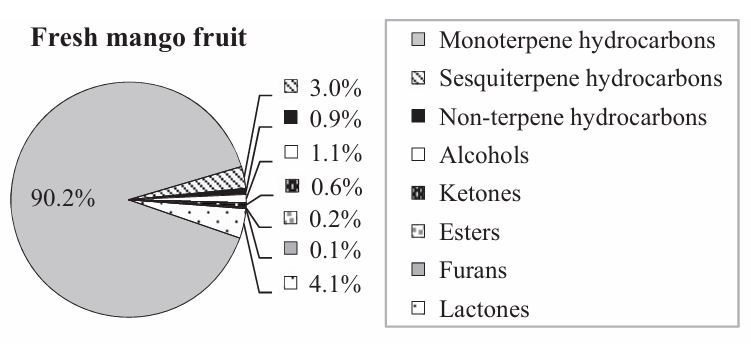
\includegraphics[width=0.8\textwidth]{Figures/fig_fresh_mango_chemical_classes.JPG}
    \caption{Distribution $[\%]$ of chemical classes of volatile compounds in fresh mango. Adapted from Bonneau et al. (2016) \cite*{A07_Bonneau2016}.}
    \label{fig:mango_aroma_compounds}
\end{figure}

\subsection{Key Aroma Compounds in Mango}
In this subsection, the key aroma compounds identified from fresh mango fruits in the study by Bonneau et al. (2016) are discussed \cite*{A07_Bonneau2016}. .

\subsubsection{Terpenes and Terpenoids}
Terpenes represent the largest class of mango aroma compounds, derived from isoprene units via the terpenoid biosynthetic pathway \cite*{A09_Barras2024}. They include both monoterpenes and sesquiterpenes, which together account for the majority of mango volatiles \cite*{A07_Bonneau2016}. Terpenes and terpenoids are found in many different natural sources, including fruits, plants, animals, microbes, and fungi. The terpenes belong to the largest class of secondary metabolites in nature and consist of five connected carbon atoms, known as isoprene units. These carbon units can be assembled in thousands of ways \cite*{B01_TerpenesTerpenoids_2018}. The terpenoids are further subcualified into five sub-groups based on the number of isoprene units they contain: monoterpenes (C10), sesquiterpenes (C15), diterpenes (C20), sesterterpenes (C25), and triterpenes (C30) \cite*{B01_TerpenesTerpenoids_2018}.

\paragraph*{Monoterpene hydrocarbons}
A total of 11 monoterpene hydrocarbons were identified as key aroma compounds in fresh mango \cite*{A07_Bonneau2016}. The most significant ones include: $\alpha$-phellandrene, $\gamma$-terpinene, $\delta$-3-carnene, $\beta$-myrcene, $\alpha$-terpinene, limonene, $\beta$-phellandrene, and $\alpha$-terpineolene. 

\vspace{1em}
Monoterpenes are the smallest molecules in the isoprenoid family with conserved hydrocarbons \cite*{A09_Barras2024}. They share the formula $C_{10}H_{16}$ and over 400 different chemical structures has been classified as such \cite*{A09_Barras2024}. The key monoterpene hydrocarbons identified in mangos are reported to have significant impact on the overall odorants \cite*{A07_Bonneau2016}.

\paragraph*{Sesquiterpene hydrocarbons}
Compared to monoterpenes, sesquiterpenes are larger molecules with the formula $C_{15}H_{24}$. In mango fruit, the study by Bonneau et al. (2016) identified four key sesquiterpene hydrocarbons, including: $\alpha$-gurjunene, $\alpha$-copaene, $\beta$-caryophyllene, and $\alpha$-caryophyllene \cite*{A07_Bonneau2016}.


\subsubsection{Alcohols and Aromatic Alcohols}
Alcohols and aromatic alcohols are, like terpenes and terpenoids, major contributors to the key aroma of mango, though they differ in chemical structure and biosynthetic origin. A study by Singh et al. (2010) highlighted the role of alcohol dehydrogenase (ADH) in the enzymatic reduction of aldehydes leading to the formation of these compounds \cite*{A10_Singh2010}.

\vspace{1em}
A total of nine alcohols were identified as volatile compounds in \textit{Kent} fresh mango \cite*{A07_Bonneau2016}. Among these compounds, 1-butanol was quantified as one of the key aroma contributors. Other identified alcohols include 3-methyl-1-butanol, 2-decanol, and 1-hexanol. Many compounds, such as 2-methyl-1-propanol did not appear in the fresh \textit{Kent} mango, but increased significantly during drying \cite*{A07_Bonneau2016}.

\subsubsection{Aldehydes and Aromatic Aldehydes}
Aldehydes are volatile compounds primarily formed through the oxidation of unsaturated fatty acids, such as $\alpha$-linolenic acid, via the lipoxygenase (LOX)-hydroperoxide lyase (HPL) pathway. These reactions generate C$_6$ and C$_9$ aldehydes, often referred to as green leaf volatiles, which are associated with fresh and grassy notes in the mango fruit aroma \cite*{A11_Sivankalyani2017}. In mango, this pathway becomes particularly active under chilling stress, leading to increased levels of compounds such as 1-hexanal, (\textit{E})-2-hexenal, and (\textit{Z})-3-hexenal before visible quality loss occurs.

\vspace{1em}
In the fresh \textit{Kent} mango, a total of one aldehyde, hexanal, was identified as key aroma compounds \cite*{A07_Bonneau2016}. While not detecable in the fresh fruit, the study did identify a total of six aldehydes post-drying, include hexanal, (\textit{E,E})-2,4-heptadienal, nonanal, and (\textit{E,Z})-2,4-heptadienal \cite*{A07_Bonneau2016}.

\subsubsection{Lactones}
Lactones are VOCs that quantitatively represents a smaller fraction of the mango aroma profile compared to terpenes and terpenoids. They are nonetheless important contributors to the overall sensory experience of the fruit, and make up two times the quantitative amount of alcohols, ketones, esters, and furans combined \cite*{A14_Silva2021, A07_Bonneau2016}. Lactones are cyclic esters formed through the intramolecular esterification of hydroxy acids. In mango, they are primarily derived from the oxidation and subsequent cyclization of fatty acids during the ripening process \cite*{A13_ElHadi2013}.

\vspace{1em}
A total of five lactones were identified as volatile compounds in fresh mango, in the study by \textcite*{A07_Bonneau2016}. Among these compounds, the most significant constituent in the fresh fruit was $\gamma$-butyrolactone. Other lactones detected includes: $\alpha$-methyl-$\gamma$-bytyrolactone, $\gamma$-hexalactone, $\delta$-hexalactone, and $\delta$-ocatlacetone \cite*{A07_Bonneau2016}.

\subsubsection{Minor Volatile Compounds: Ketones, Esters, and Furans}
Ketones, esters, and furans are present in much smaller amounts compared to terpenes and terpenoids, but still contribute to the complexity of mango aroma \cite*{A07_Bonneau2016}. Ketones are important volatile compounds that can be identified in exotic fruits such as mango, e.g. 1-octen-3-ona, which provides a mushroom aroma \cite*{A01_Aguirre-Lopez_2023}. Esters are associated with fruity and sweet nuances, whereas the furans provide the mango fruit with mild caramel-like notes. Despite low abundance of these three classes of compounds, they may enhance the overall balance of aroma perception in fresh mango \cite*{A13_ElHadi2013}.

\subsection{Variation in Aroma Profiles Among Mango Varieties}
The volatile composition of mango (\textit{Mangifera indica} L.) varies substantially among cultivars, reflecting genetic differences and environmental influences on fruit metabolism and ripening \cite*{A01_Aguirre-Lopez_2023}. Comparative analyses of multiple mango varieties have shown that the abundance and composition of key aroma compounds differ significantly across cultivars, leading to distinct sensory profiles \cite*{A01_Aguirre-Lopez_2023,A02_Moreno2010}. 

\vspace{0.5em}
A recent study by \textcite{A16_Tandel2023} investigated sixteen Indian mango cultivars, revealing notable differences in their volatile profiles. Cultivars such as \textit{Alphonso}, \textit{Kesar}, and \textit{Ratna} were characterised by high levels of terpenes, whereas \textit{Amrapali} was dominant in esters \cite*{A16_Tandel2023}. Within the terpene class, \textit{allo-ocimene} and $\beta$-ocimene were frequently dominant, while the presence of butanoic acid derivatives contributed to the sweeter aroma of ester-rich cultivars \cite*{A16_Tandel2023}. 

\vspace{0.5em}
\textcite{A13_ElHadi2013} further distinguished the aroma profiles of mango cultivars according to their geographical origin. New World varieties, such as \textit{Haden}, \textit{Irwin}, and \textit{Tommy Atkins}, were typically dominated by terpene hydrocarbons—especially $\delta$-3-carene—whereas Old World cultivars contained higher proportions of esters, alcohols, and ketones, resulting in sweeter and fruitier profiles \cite*{A13_ElHadi2013}. 

\vspace{0.5em}
As discussed by \textcite{A16_Tandel2023}, previous studies comparing Chinese cultivars \textit{Tainong} and \textit{Jinmang} found high levels of $\beta$-ocimene, myrcene, and $\alpha$-terpinolene, which significantly contributed to their aroma profiles. These results aligned with \textcite{A15_Xie2023}, who also reported terpenes as a dominant volatile class in \textit{Jinmang}. In a separate comparison of \textit{Tainong} and \textit{Hongyu}, \textcite{A15_Xie2023} observed that \textit{Tainong} had higher levels of terpenes and aldehydes, producing a grassy aroma, while \textit{Hongyu} exhibited higher ester content, leading to a more fruity and sweet aroma.


\section{Biochemical Pathways of Aroma Compound Formation}
VOCs are low-molecular-weight molecules with functional groups such as alcohols, esters, ketones, aldehydes, and terpenes \cite*{A01_Aguirre-Lopez_2023,B01_TerpenesTerpenoids_2018}. These compounds are synthesised through metabolic and enzymatic reactions during maturation and ripening, and significantly impacts the fruits aroma profile \cite*{A01_Aguirre-Lopez_2023}. VOC profiling is therefore an important indicator of fruits quality, cultivar differentiation, and ripeness \cite*{A01_Aguirre-Lopez_2023}. 

\vspace{1em}
The study of VOCs is known as \textit{volatilomics}, which investigates the biosynthesis and metabolic pathways of aroma compounds \cite*{A01_Aguirre-Lopez_2023}. The biosynthesis of VOCs in fruits is based on three major pathways: the amino acid derivative pathway, the fatty acid derivative pathway, and the terpenoid pathway \cite*{A13_ElHadi2013}. These pathways will be described in detail below. Once the basic molecular forms are synthesised, enzymatic reactions, such as hydroxylation, acylation, methylation, oxidation-reduction, and ring closure, enhance volatility and molecular diversity \cite*{A13_ElHadi2013}.


\subsection{Enzymes Involved in Aroma Biosynthesis}
The diversity of VOCs in mango arises from enzymatic reactions that modify basic molecular structures, e.g. hydroxylation, acylation, methylation, oxidation-reduction, and ring closure \cite*{A13_ElHadi2013}. ADH plays a key role in converting aldehydes to alcohols and supplies substrates for ester synthesis. Mangoes expresses multiple ADH isoforms (MiADH1-3) that are differentially regulated during ripening \cite*{A10_Singh2010}. Other enzymes which contributes to the aroma formation includes methionine $\gamma$-lyase and 3-ketoacyl-CoA thiolase B, which are active in amino-acid- and fatty-acid-derived pathways \cite*{A05_Chin2019}. In the fatty acid pathway, LOX and HPL cooperates with ADH to produce $C_6$ and $C_9$ volatiles, whereas terpene synthases (TPSs) catalyses the cyclisation of prenyl diphosphate precursors in the terpenoid pathway \cite*{A13_ElHadi2013}.


\subsection{Amino Acid Derivative Pathway}
The Amino Acid Derivative Pathway is responsible for synthesizing the fruits characterised flavour and aroma compounds \cite*{A13_ElHadi2013}. Amino acids, such as alanine, valine, leucine, isoleucine, phenylalanine, and aspartic acid, serves as direct precursors for these pathways, forming a variety of compounds including alcohols, carbonyls, acids, and esters \cite*{A13_ElHadi2013}. The biosynthesis typically starts with a deamination or transamination reaction that produces the corresponding $\alpha$-keto acid \cite*{A13_ElHadi2013}. Subsequent steps follows, including decarboxylation, reduction, oxidation, and/or esterification, to produce the volatile compounds \cite*{A13_ElHadi2013}, e.g. branched chain volatiles, which often are derived from leucine, isoleucine, and valine \cite*{A05_Chin2019}.


\subsection{Fatty Acid Derivative Pathway}
The fatty acid derivative pathway is a major source of aroma volatiles in fruits. The pathway produces straight-chain alcohols, aldehydes, ketones, esters, and lactones \cite*{A13_ElHadi2013}. There are mainly three processes involved in the fatty acid derivative pathway: $\alpha$-oxidation, $\beta$-oxidation, and the LOX pathway \cite*{A13_ElHadi2013,A16_Tandel2023}. The $\beta$-oxidation process shortens fatty acids by removing $C_2$ units (acetyl-CoA), forming precursors for ester synthesis \cite*{A13_ElHadi2013}. The LOX pathway converts polyunsaturated fatty acids such as linoleic and linolenic acid into $C_6$ and $C_9$ aldehydes and alcohols via HPL and ADH \cite*{A13_ElHadi2013}. Compounds like hexanal and nonanal are formed by linolenic and oleic acid degradation, and hydroxylated intermediates can undergo spontaneous lactonization to form lactones such as $\gamma$-butyrolactone \cite*{A07_Bonneau2016,A14_Silva2021}.


\subsection{Terpenoid Pathway (MEP and MVA Pathways)}
Terpenoids represent the largest class of plant secondary metabolites, the two primary groups are monoterpenes and sesquiterpenes \cite*{A04_GUO2023112779, A02_Moreno2010, A09_Barras2024}. They all share the $C_5H_8$ isoprenoid unit and are derived from the universal precursors isopentenyl diphosphate (IPP) and dimethylallyl diphosphate (DMAPP), and are synthesised by two distinct routes: the cytosolic mevalonic acid (MVA) pathway, and the plastidial methylerythritol-4-phosphate (MEP) pathway \cite*{A09_Barras2024,A13_ElHadi2013}. MVA starts from acetyl-CoA, whereas MEP uses pyruvate and glyceraldehyde-3-phosphate (G3P) as precursors \cite*{A09_Barras2024}. These pathways happens simultaneously in different cellular compartments, enabling an exchange of intermediates \cite*{A09_Barras2024}. Subsequently, IPP and DMAPP are joined together by prenyltransferases which produces geranyl pyrophosphate (GPP) and farnesyl pyrophosphate (FPP) \cite*{A09_Barras2024,A13_ElHadi2013}. TPSs then catalyses the cyclisation into different terpene skeletons that defines the mango aroma \cite*{A09_Barras2024,A13_ElHadi2013}.


\section{Environmental and Genetic Factors Influencing Aroma Production}
The aroma profile of fruit is complex and determined by a combination of both genetics and environmental factors \cite*{A13_ElHadi2013,A16_Tandel2023}. The composition and concentration of VOCs are specific to the fruit species and across cultivars \cite*{A13_ElHadi2013,A16_Tandel2023}. Variations among mango cultivars, for example, demonstrate that genetic background defines the abundance of specific volatile classes (e.g., some are monoterpene-dominant, while others has high levels of esters, fatty acids, or sesquiterpenes) \cite*{A16_Tandel2023}.


\subsection{Pre-harvest Factors}
Pre-harvest conditions significantly influence the final volatile composition \cite*{A13_ElHadi2013}. Environmental conditions such as climate (temperature and humidity) and geographic region (sunlight, precipitation, and fertilisation) can modulate VOC quantity in plants \cite*{A01_Aguirre-Lopez_2023,A16_Tandel2023}. These factors affect crop growth and aroma quality, including flavour and texture \cite*{A13_ElHadi2013}. 


\subsection{Post-harvest Factors}
The stage of maturity and ripening is a critical post-harvest factor since VOCs are released during the maturation processes \cite*{A01_Aguirre-Lopez_2023,A13_ElHadi2013}. In climacteric fruits like mango, ripening is associated with an increase in ethylene production and subsequent synthesis of aromatic volatiles \cite*{A05_Chin2019}. In mango, the expression of key aroma genes, such as ADH, is regulated by hormones like ethylene and Abscisic Acid (ABA) at the initial stages of ripening \cite*{A10_Singh2010}. Furthermore, storage temperature has a significant impact on the volatile profile \cite*{A13_ElHadi2013}. Storing mangoes at sub-optimal temperatures (e.g.5\textdegree C) induces chilling stress, which results in a reduced formation of desirable aroma compounds such as monoterpenes, while it simultaneously increases $C_6$ and $C_9$ aldehydes \cite*{A11_Sivankalyani2017}.


\subsection{Processing Implications on Aroma Retention}
Processing methods, particularly drying, results in a significant loss of aroma compounds \cite*{A07_Bonneau2016}. A study by \textcite{A07_Bonneau2016} on drying \textit{Kent} mango fruit showed a total volatile loss of approximately 58.8\% \cite*{A07_Bonneau2016,A16_Tandel2023}. This decline is primarily attributed to evaporation and thermal degradation of compounds such as monoterpenes, sesquiterpenes, and lactones \cite*{A07_Bonneau2016}. However, pretreatment techniques like osmotic dehydration (DO) has shown to help decrease these losses and aid in the conservation of volatile compounds \cite*{A02_Moreno2010}. It was proposed that sugar impregnation blocked the exit of internal gases during subsequent drying \cite*{A02_Moreno2010}. Some compounds, such as hexanal and nonanal, showed a post-drying increase possibly due to the degradation of unsaturated fatty acids \cite*{A07_Bonneau2016}.


\section{Analytical Techniques for Aroma Compound Identification}
\subsection{Extraction and Analysis Methods}
The most common technique for sampling volatile compounds in fruits is Solid Phase Microextraction (SPME) \cite*{A01_Aguirre-Lopez_2023}. SPME is highly favored because it is solvent-free, fast, sensitive, and requires minimal sample manipulation by reliably collecting analytes from the headspace (HS) \cite*{A01_Aguirre-Lopez_2023,A03_PanoFarias2017}. The technique typically utilizes adsorbent fibers composed of materials such as DVB, CAR, PDMS, and PA to capture the volatile compounds \cite*{A01_Aguirre-Lopez_2023}. When extracted, the Gas Chromatography coupled with Mass Spectrometry (GC-MS) is used, which separates molecules and identifies them via mass detection \cite*{A01_Aguirre-Lopez_2023}. Other used methods include Liquid-Liquid Extraction (LLE) for non-polar VOCs \cite*{A01_Aguirre-Lopez_2023}, Solvent Assisted Flavour Evaporation (SAFE) for preparing aroma extracts of the original product \cite*{A01_Aguirre-Lopez_2023}, and Single Drop Microextraction (SDME) for miniaturized analysis \cite*{A03_PanoFarias2017}.


\subsection{Quantification and Sensory Evaluation}
Sensory analysis is a crucial aspect. Odour and aroma are quality attributes directly linked to consumer acceptance \cite*{A01_Aguirre-Lopez_2023}. To quantify the sensory impact, the Odor Activity Value (OAV) estimates odor potency by calculating the ratio between a compound's concentration and its odor detection threshold \cite*{A01_Aguirre-Lopez_2023,A07_Bonneau2016}. Similarly, Aroma Extract Dilution Analysis (AEDA) can rank the perception of compounds which are important to the overall aroma via the flavor dilution (FD) factor \cite*{A01_Aguirre-Lopez_2023,A07_Bonneau2016}. Specialized techniques combines analysis with human perception, such as GC-Olfactometry (GC-O), which routes the column effluent to a "sniffing port" for sensory evaluation by a trained panel \cite*{A01_Aguirre-Lopez_2023}. Furthermore, Multivariate Data Analysis, such as Multiple Correspondence Analysis (MCA), is used to explore statistical correlations between molecules, aromas, and fruits \cite*{A01_Aguirre-Lopez_2023,A15_Xie2023}.


\section{Comparative Perspective}
Mango aroma varies significantly across cultivars, geography, and processing, indicating both genetic and environmental influences on volatile biosynthesis \cite*{A13_ElHadi2013,A16_Tandel2023}. Indian cultivars showed differences like \textit{Alphonso}, \textit{Kesar}, and \textit{Ratna} which often are terpene-dominant, while other cultivars exhibited different major components, such as \textit{Neelum} which had high levels of sesquiterpenes (74.80\%) \cite*{A16_Tandel2023}. Geographical factors also showed significant variations. New World varieties (\textit{Haden} and \textit{Tommy Atkins}) were dominated by terpene hydrocarbons, while Old World mangoes contained higher proportions of esters, alcohols, and ketones \cite*{A13_ElHadi2013}. Similarly, analysis confirmed that \textit{Tainong} expressed grassy notes due to high terpene and aldehyde content, while \textit{Hongyu} was rich in esters and were perceived as fruity and sweet \cite*{A15_Xie2023}.

\vspace{1em}
Ripening and post-harvest handling significantly impacts the aroma profiles. During maturation, ethylene activation enhances the synthesis of aromatic volatiles, including terpenes and esters derived from pathways involving ADH \cite*{A10_Singh2010}. Conversely, chilling stress (e.g., storage at 5\textdegree C) compromises aroma quality by suppressing monoterpenes and increasing the concentration of stress-related $C_6$ and $C_9$ aldehydes and alcohols \cite*{A11_Sivankalyani2017}. Drying \textit{Kent} mangoes greatly reduces the total volatile content, mainly through the loss of terpenoids, but compounds like lactones and esters may be retained or enriched, altering the sensory balance \cite*{A07_Bonneau2016}. Techniques like osmotic dehydration has been proposed to help mitigate these losses \cite*{A02_Moreno2010}.

\vspace{1em}
The variation observed in aroma studies is often attributed to the analytical choices, as the volatile profile is highly sensitive to the method used \cite*{A13_ElHadi2013}. Techniques such as SPME, SDME, and SAFE capture different classes of compounds from the fruit headspace \cite*{A01_Aguirre-Lopez_2023,A07_Bonneau2016}. Crucially, GC-O, often utilizing flavor dilution analysis, identifies compounds based on their potent sensory impact, such as a high OAV, rather than only their chemical abundance recorded by GC-MS \cite*{A01_Aguirre-Lopez_2023,A07_Bonneau2016}.


\section{Conclusion}
Mango aroma complexity stems from the interaction of hundreds of VOCs, predominantly monoterpene hydrocarbons, which originate primarily from three core biosynthetic routes: the Terpenoid pathway, the Fatty Acid Derivative pathway, and the Amino Acid Derivative pathway.

\vspace{1em}
The specific aroma profile is highly influenced by the cultivars genetic background, leading to significant differences between terpene-dominant New World cultivars and ester/alcohol-rich Old World varieties. This inherent chemistry is critically influenced by environmental and post-harvest factors. Ripening promotes the synthesis of aromatic volatiles, while stresses, such as cold storage (5\textdegree C), lead to less formation of monoterpenes and an increase in both $C_6$ and $C_9$ aldehydes from the oxidation of $\alpha$-linolenic acid. Furthermore, processing methods like drying, causes significant losses of volatile compounds, approximately 58.8\%, although pre-treatment strategies like osmotic dehydration can mitigate the aroma decrease.

\vspace{1em}
Accurate characterization of the aroma profiles relies on analytical tools, primarily SPME extraction coupled with GC-MS, complemented by sensory techniques like GC-O and OAV to identify the few odor-active compounds that define consumer perception. Comprehensive understanding of these biochemical and environmental factors are essential for the mango industry to optimize post-harvest handling and select cultivars that guarantee specific, consumer-desirable aroma traits. Future research should aim to combine volatilomics with genetic data, thereby linking the key synthesis enzymes like ADH, TPSs, and LOX to cultivar-specific aroma formation.

%\chapter{Product Concept}
\setlength{\headheight}{22.94003pt}
\addtolength{\topmargin}{-10.22661pt}

\section{Product Concept}
It is estimated that only 35\% of the globally produced plant protein is consumed by humans. Meanwhile the current market offers a wide range of plant-based proteins available which are well fitted for human consumption. Common choices include formulations with oat, wheat, hemp, soy and pea to name a few (Gorissen et al., 2018). The Cannabis sativa L., a Cannabaceae known as ‘‘hemp’’ is of increasing interest because it is highlighted as an environmentally friendly and economically high-potential crop. Its history as a source for medicine, fiber and food dates back 6000 years, and the cultivation of hemp with close to no levels of tetrahydrocannabinol (THC), the psychoactive compound found in cannabis, has increased to use in foods since strains with a THC content below 0.3\% was approved in EU in 1996. Among its many advantages are fast growth and low dependency on pesticides, which benefits biodiversity and healthy soils. Furthermore, its seeds provide a valuable source of nutrients. (Chapter 6 Industrial Hemp Seed). Globally, the trend of increasing interest for hemp seeds is clear, as the production increased from 2,718 tons to 5,449 tons between 2015 and 2020. 

\vspace{1em}
Thus, developing a convenient hemp-based bar would harness the many benefits of the not-so-novel ingredient that is hemp seed. Below is a mock up of the Hemp Protein Bar (figure 4).

\begin{figure}[H]
    \centering
    \includegraphics[width=0.54\linewidth]{Figures/fig_prod_concept_01.png}
    \caption{AI-generated illustration of a medieval marketplace. Generated using DALL·E 3 (OpenAI, 2025) with the prompt: "Mock up of a hemp bar picture half coved in chocolate ".}
    \label{fig:prod_concept_01}
\end{figure}


\subsection{Macronutrients in Hemp Seeds}
Hemp seeds typically contain around 20-30\% protein, 25\%-35\% lipids, 20-30\% carbohydrates and 4-7\% of ash (Figure 5). It has a balanced composition with particularly low starch content. (Montero et al 2023) 

\begin{figure}[H]
    \centering
    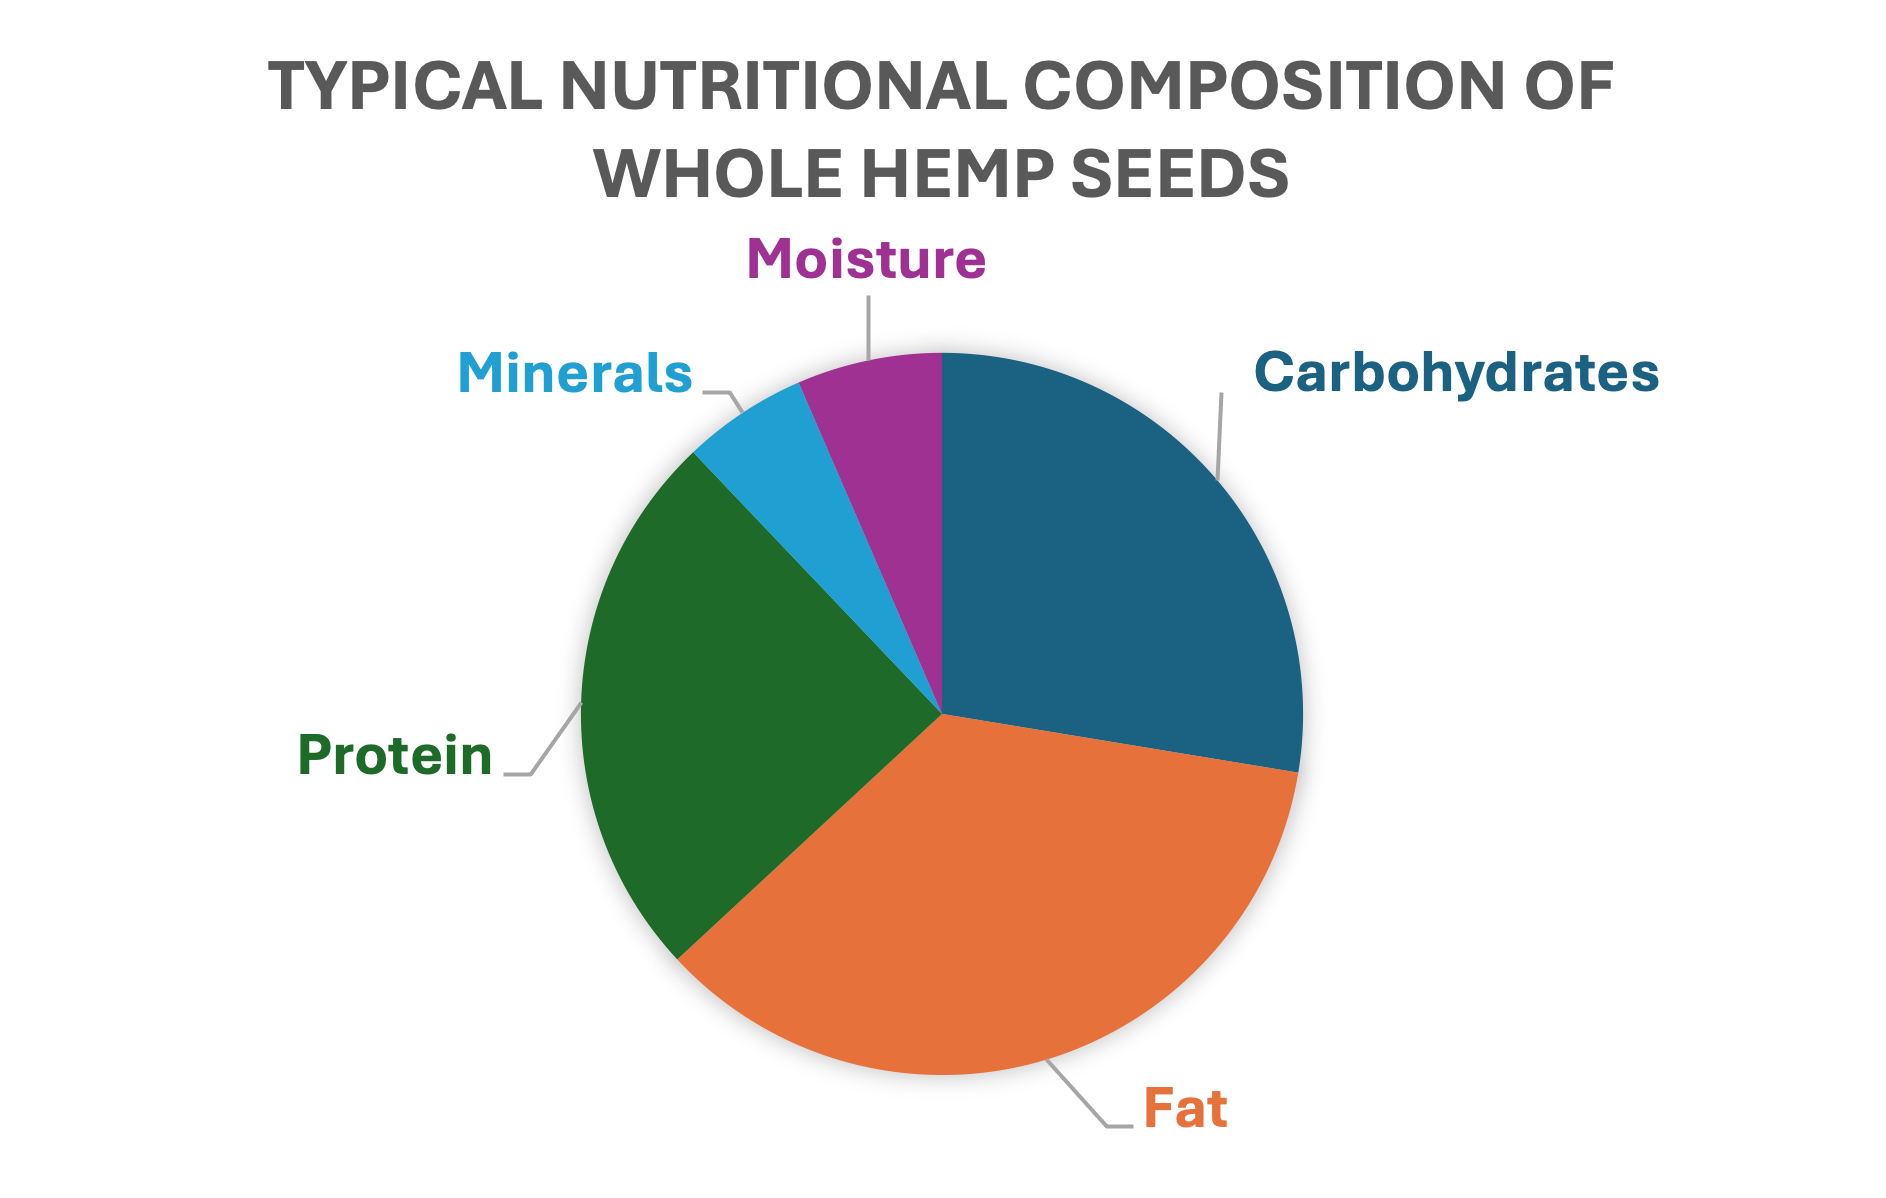
\includegraphics[width=0.75\linewidth]{Figures/fig_prod_concept_02.png}
    \caption{Composition diagram of whole hemp seeds}
    \label{fig:prod_concept_02}
\end{figure}

\subsubsection{Protein}
Hemp seeds are an excellent source of high-quality protein, typically containing 20–30\% protein, with dehulled hemp seeds having even higher protein contents, ranging from 30\% to 38\%. (chapter 4 hemp seed book). The two main proteins in hemp seeds are albumin (33\%) and edistin (65\%), which have very similar structures to plasma proteins which helps the digestibility in humans. Hemp seeds provide a complete amino acid profile, containing all nine essential amino acids required by humans, making them comparable to other high-quality proteins like egg white and soybeans (Chapter 10). 

\vspace{1em}
The protein is also particularly rich in arginine, glutamic acid, and aspartic acid, where arginine is especially valuable as it is a precursor to nitric oxide, which enhances blood flow and helps maintain normal blood pressure, contributing to cardiovascular health (chapter 11 hemp book)
Hemp proteins are highly digestible, with dehulled hemp seeds demonstrating superior protein digestibility (83.5–92.1\%) (hemp nutritional value). This is partly attributed to the absence of protease inhibitors in hemp seeds (Hemp seed bioactivity). 

\vspace{1em}
A study has analysed the macronutrient composition and protein quality of 30 hemp seed products from Western Canada, including whole seeds, dehulled seeds, and hemp seed meal. Crude protein, fat, and amino acid profiles were determined, and protein quality was assessed using the Protein Digestibility-Corrected Amino Acid Score (PDCAAS) method, based on a rat bioassay and FAO/WHO amino acid requirements for young children. Average protein content ranged from 24.0\% in whole seeds to 40.7\% in hemp seed meal. Protein digestibility was 84–98\%, with protein digestibility-corrected amino acid score (PDCAAS) values of 46–66\%, highest in dehulled seeds. The protein digestibility-corrected amino acid score of dehulled hemp seed is comparable to lentils and is about half that of casein, and almost twice that of almonds (chapter 10 hemp seed book)

\subsubsection{Fatty Acids}
Hemp seed oil is primarily composed of polyunsaturated fatty acids, PUFA (over 80\%) including fatty acids like essential linoleic acid (omega-6) and alpha-linolenic acid (omega-3). (Chapter 10 hemp seed book) Dehulled hempseeds have a healthy balance of omega-6 to omega-3 polyunsaturated fatty acids (2.5:1) (Chapter 1 hemp book)

\vspace{1em}
Unsaturated fatty acids help protect against cardiovascular disease, obesity, diabetes, and inflammation. EFSA recommends an optimal omega-6/omega-3 ratio of 3:1 to 5:1. Hemp seed oil typically shows a ratio of 2.5–3.5:1, which is a desirable range linked to lower chronic disease risk. (Hemp nutritional value pdf)

\subsubsection{Carbohydrates}
About 98\% of the carbohydrates in hemp seeds are dietary fiber, mainly insoluble dietary fibers (80\%), such as cellulose, lignin and hemicellulose. Dietary fiber resists enzymatic digestion in the small intestine and undergoes partial or complete fermentation in the large intestine. The remainder of the carbohydrates in hemp seeds is starch. Therefore, hemp seeds are considered a low-starch food and an excellent source of dietary fiber. (Hemp nutritional value pdf) 

\vspace{1em}
The dietary fibers from hemp seeds are associated with positive effects on the digestive tract support by acting as prebiotics. The fermentation of fibers in the colon generates short-chain fatty acids that have beneficial roles in the body. (Hemp seed bioactivity pdf). In the Western countries the consumption of dietary fiber is lower than the recommended intake, making hemp seeds an attractive ingredient to meet the recommended daily intake of dietary. However, processing might affect the amounts of dietary fibers in hemp seeds. 

\subsection{Micronutrients: Vitamins and Minerals}
Hemp seeds are rich in vitamins and minerals. Just 50 mg of hemp seed can supply at least half of the recommended daily allowance of copper, magnesium, and zinc, and exceed the recommended daily allowance of the vitamins A, D, and E. (Chapter 1 hemp book) Hemp seeds also contain other micronutrients such as phosphorus, potassium, calcium, sodium, iron, and manganese. (Chapter 4 hemp book). Hemp seed oil contains fat-soluble vitamins, in particular vitamin E (tocopherols) and vitamin A which respectively has an antioxidant role and is beneficial for skin integrity and Vitamin D is important for bone health and the immune system (Hemp nutritional value pdf)

\vspace{1em}
Besides the macro- and micronutrients, secondary metabolites, such as terpenes, phytosterols and flavonoids, constitute essential components of the defence response of the hemp plant to biotic and abiotic stresses. However, the composition of these secondary metabolites can be influenced by cultivation conditions, providing a distinct fingerprint of different production regions. It is suggested that these compounds contribute with antioxidative, antimicrobial, and anti-inflammatory properties in the human body. Phytosterols for instance, are not synthesized in humans, but can when ingested from plants, reduce cholesterol levels in the human body by changing the cholesterol solubility in the intestine. (Tănase et al. 2024).

\subsection{Potential Side Streams}
The industrial hemp plant has a versatile plant body which consists of seeds, leaves, stem, and flowers with several application opportunities depending on the part of the plant. Particularly the stem is a valuable source to produce hemp fiber which can be used for rope, building materials, paper, or textiles. The seeds, dehulled or whole, can be utilized as a food source. The hemp flower can be used to produce cosmetic and pharmaceutical products, including essential oils. When looking further into hemp as a natural source to bast fiber a life cycle assessment reveals that hemp performs better than glass fiber by weight and compared to cotton, hemp requires less water and pesticides to grow although hemp fiber is known to be coarser and stiffer than cotton which has a softer appearance. (Kaur \& Kander 2023). 

\vspace{1em}
When processing the stem to hemp fiber a by-product of shives is made. It can be used to produce hemp concrete which is a bio-composite and carbon-negative alternative to concrete for construction and insulation. (Yano \& Fu 2023). These useful side streams make hemp even more attractive to use as an ingredient in foods. 

\subsection{Dietary Pattern of the Chosen Consumer Group and Product Fit}
Our hemp seed bar is uniquely positioned to seamlessly integrate into several contemporary dietary patterns, directly addressing the needs and preferences of our diverse target consumer groups within the Millennial and Generation Z age group.

\vspace{1em}
For vegetarians and vegans dehulled hemp seeds are an excellent source of high-quality, plant-based protein. The seeds naturally contain all nine essential amino acids required by humans, offering a complete protein profile that can be challenging to obtain from other plant sources. (Chapter 1 hemp seed book) The protein in dehulled hemp seeds also boasts superior digestibility (83.5\%-92.1\%) compared to whole hemp seeds and hemp meal, making its nutrients more accessible. They also provide a healthy balance of omega-6 to omega-3 polyunsaturated fatty acids (typically 2.5:1 to 3.5:1), which is desirable for overall human nutrition. (Hemp nutritional value pdf) Hemp protein and flour can serve as an alternative for soy ingredients (Chemical composition and biological activities of PDF) 

\vspace{1em}
A health-conscious person or athlete would also use it for its excellent source of protein, especially because of the high value protein composition with the nine essential amino acids. Furthermore, it scores high in terms of digestibility which makes our bar effective for muscle recovery and satiety. (Chapter 10 hemp book) Many athletes need to have control on their calorie needs. Our bar could therefore be an easy boost of calories or be used as a substitute for a snack or meal.
\vspace{0.5em}
The bar is rich in healthy fats, including the beneficial omega-6 to omega-3 ratio, which is important for cardiovascular health and may help prevent chronic diseases. (Hemp nutritional value pdf)

\vspace{1em}
Our bar is also a good source of essential minerals like copper, magnesium, and zinc, and provide vitamins A, D, and E, which also talks to the health-conscious person (Chapter 1 hemp book)

\vspace{1em}
For individuals with dietary restrictions and/or allergies our bar is also a great option, as our bar is naturally gluten-free, making it a safe nutritious option for people with celiac disease or gluten sensitivities. (Chapter 1 hemp book) Hemp proteins are generally considered to have low allergenicity compared to common proteins like soy, dairy, or wheat, broadening its appeal for those with various food allergies. (Chapter 11 hemp book \& Hemp nutritional value pdf)

\vspace{1em}
For environmentally aware consumers our hemp-based product directly supports environmental sustainability due to it having a low environmental impact, actively contributing to improved soil health, water quality, have carbon-negative crops and requiring no or little pesticide use. (Chapter 1 hemp book \& hemp nutritional value PDF \& hemp seed bioactivity) 

\vspace{1em}
The pre-packaged protein bar format offers convenience and time efficiency, requiring no preparation or cleanup for the people on-the-go. It delivers the balanced nutrition derived from dehulled hemp seeds in an easily consumable form, perfectly fitting the needs of busy individuals seeking healthy and convenient dietary options.



%%\chapter{Formulation and Raw Materials}
\setlength{\headheight}{12.71342pt}
\addtolength{\topmargin}{-0.71342pt}

\section{Formulation and Raw Materials}
The formulation of the hemp seed bar is an important factor, as it regulates the final nutritional composition and determines the parameters for the upstream and downstream processing steps. Using consistent suppliers and high-quality raw materials are key factors in maintaining a predictable, consistent production. Production as such would decrease faults, which reduces waste and ensures safe a safe high-end product to the final consumer. 

\vspace{1em}
Given the lack of sweetness of hemp seeds, the bar is formulated with naturally sweet components such as dried dates and agave sirup. Along with a caramelly flavor, important cohesiveness of the bar is achieved. The dates are dried which reduces water content and thus increases sugar concentration and intensifies flavor. Minimum processing other than dehydration and pitting ensures valuable components such as micronutrients and fibers are included.

\vspace{1em}
To complement the protein value (which lacks in lysine), potato protein isolate is used. During its production, it undergoes heavy processing which concentrates the protein content while reducing other macronutrients, minerals and vitamins (Wagley et al., 2019).

\vspace{1em}
Rolled oats are used as a structural component. It is chosen as it is a gluten free, cheap, readily available raw material known to consumers. It undergoes dehulling, rolling and steaming, which maintains the high fiber content while inactivating lipase enzymes to prevent oxidation and extend shelf life (Ekelund et al., 2024). Ground flax seeds are also included to account for the loss of dietary fibers in Hemp. The flax seeds are grounded to inhibit toxic effects of cyanogenic glycosides (Nowak et al., 2023).

\vspace{1em}
Preprocessing of hemp seeds aims to partially remove the hull/husk (figure 6). The macronutrient profile of the seed is significantly affected by the processing method. Although the formulation does not involve hemp protein isolate, HPI, many studies on this subject point at the effects of preprocessing. 

\vspace{1em}
For example, a study by House et al., 2010 evaluated HPI derived from whole seeds, hemp seed meal, and solely hulls. The study could show that the amino acid composition is different among the three processed raw materials. In the works by Shen et al., 2020 the HPI of dehulled and whole seeds were comprehensively investigated in terms of aromatic components, colour, and protein characterization. Dehulled seeds would increase the extraction yield by 21.52 \% and protein recovery yield (46.90\%) of the HPI. Naturally, the HPI with whole seeds would contain increased amounts of lipids and carbohydrates. The preprocessing also had a profound impact on colour, were whole seeds generated a darker coloured HPI. This matter is further explained in the section “4.1 Effects on Processing”

\vspace{1em}
Vanilla extract, cocoa and sea salt are used to characterize the aroma of the bar. Potentially masking some of the earthy off-flavours from the other ingredients. 


\begin{figure}[h]
    \centering
    \begin{subfigure}{0.45\textwidth}
        \centering
        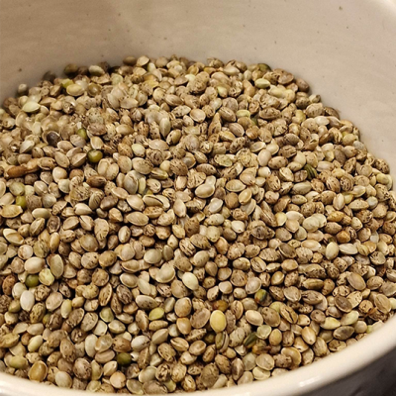
\includegraphics[width=\linewidth]{Figures/fig_formulation_06.png}
        \caption{Whole hemp seeds}
        \label{fig:whole_hemp}
    \end{subfigure}
    \hfill
    \begin{subfigure}{0.45\textwidth}
        \centering
        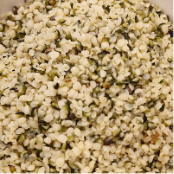
\includegraphics[width=\linewidth]{Figures/fig_formulation_06.1.png}
        \caption{Dehulled hemp seeds}
        \label{fig:dehulled_hemp}
    \end{subfigure}
    \caption{Whole and dehulled hemp seeds (Svensk Hampaindustri, 2025).}
    \label{fig:whole_dehulled}
\end{figure}


%%\chapter{Processing and Manufacturing}
\setlength{\headheight}{12.71342pt}
\addtolength{\topmargin}{-0.71342pt}

\section{Processing and Manufacturing}
The production process of the protein bar can be seen on Figure 7.
\begin{figure}[H]
    \centering
    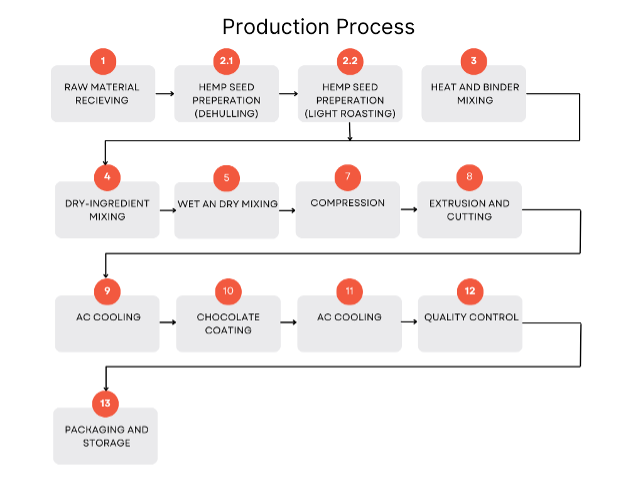
\includegraphics[width=0.8\textwidth]{Figures/fig_process_01.png}
    \caption{A flowchart with a visualization of the production process of the hemp protein bar}
    \label{fig:process_flow_diagram}
\end{figure}

\textit{Sourcing and preparing} raw materials – all ingredients are inspected for quality and stored under appropriate conditions to maintain freshness. All ingredients are weighed and portioned accurately according to the recipe formulation, ensuring batch-to-batch uniformity. This ensures that only safe, high-quality, and properly measured ingredients enter the mixing stage, laying the foundation for a consistent protein bar in terms of flavor, texture, and nutritional profile.

\vspace{1em}
\textit{Dehulling hemp seed} – Increases absorption of proteins and nutrients.

\vspace{1em}
\textit{Light roasting} – of the dehulled hemp seed (75°C-80°C) - improves digestibility, and reduces anti-nutritional factors and lower microbial load.

\vspace{1em}
\textit{Mixing} to homogeneous mixture – evenly distributed throughout the mixture providing a consistent texture and flavor in every bar. Time and temperature in mixing are controlled to ensure that every batch is consistent.

\vspace{1em}
\textit{Compression} – shaping the mixture into a form that is suitable for further processing. Using large presses ensures a uniform sheet, which helps create consistency in texture and flavor throughout the bar.

\vspace{1em}
Extrusion and cutting – A combination of extrusion and cutting technologies are used to shape the mixtures into bars. The extrusion process forces the mixture through a die, after which a knife cuts the long bars into the desired length.

\vspace{1em}
AC cooling – is used to ensure that the bar maintains the desired temperature throughout the process, as mixing and pressure from extrusion can increase the temperature of the product.

\vspace{1em}
Chocolate coating – for flavour.

\vspace{1em}
\textit{AC cooling} – to solidify the chocolate.

\vspace{1em}
\textit{Quality control} – Both automated sensors and visual inspection for defects or foreign objects. Taking samples to ensure that our product meets quality standards, as well as for example checking that the product contains enough protein to be claimed as a product with a high protein content. 

\vspace{1em}
\textit{Packaging} – wrap each bar individually and in a material that keeps the protein bar safe and to ensure that the bar does not undergo oxygenation and to preserve freshness. This process also includes labelling and coding to ensure traceability and compliance with regulatory requirements.

\subsection{Effects on Processing}
Hemp seeds contain several antinutritional, such as phytic acid, tannins and saponins. The presence of tannins and saponins can reduce the bioavailability of nutrients and disrupt both metabolism and digestive functions (kapitel 4 hampbog). The presence of phytic acid can lead to mineral deficiencies (e.g. iron, zinc and calcium), as it can inhibit the absorption of these. (kapitel 10 hampbog). Polyphenols, of which tannins are a part, are often found in the shell of hemp seeds (hemp nutritional value pdf). The same applies to phytic acid. Studies have shown that there is significantly more phytic acid present in whole hemp seeds 3.5 g/100g compared to 2.1 g/100g in hulled hemp seeds. That is a reduction of 40\%. (kapitel 4 hampbog).

\vspace{1em}
According to House et al. (2010), whole hemp seeds have a protein digestibility of approximately 84–86\% and a protein digestibility-corrected amino acid score (PDCAAS) value of 49–53\%, while dehulled hemp seeds reach a digestibility of 91–97\% and a PDCAAS value of 63–66\%. This improvement is primarily due to the fact that the hull contains a large part of the fiber fraction of the seed, which inhibits digestibility, so when the hull is removed, the fiber content is significantly reduced, making the protein more available and thus improving the overall protein assessment (PDCAAS) (Evaluating the Quality of Protein from Hemp Seed pdf.) Therefore, by using a majority of dehulled hemp seeds instead of whole hemp seeds, we reduce the content of antinutrients and increase the nutritional quality of the protein.

\vspace{1em}
Plant proteins naturally contain antinutritional factors such as trypsin inhibitors, glucosinolates, phenols and phytates, together with a high content of dietary fiber, which can negatively affect protein and amino acid digestibility and bioavailability. Heat processing can effectively help to remove or reduce these compounds, leading to higher protein digestibility. However, high heat treatment can have negative effects as it can affect the chemical transformations of amino acids. Some amino acids, such as lysine, can be chemically transformed and become unavailable during heat treatment or other severe processes, leading to problems such as the formation of Maillard reaction products. This underlines the need for appropriate processing conditions to avoid such. (Protein Quality Report No 92 web version .pdf)



\begin{table}[h]
    \centering
    \caption{Protein digestibility-corrected amino acid scores of hemp protein sources in comparison to other food proteins. (Evaluating the Quality of Protein from Hemp Seed pdf.)}
    \label{tab:process_table_01}
    \begin{tabular}{l c}
    \hline
    \textbf{Protein source} & \textbf{PDCAAS (\%)} \\
    \hline
    Casein               & 100 \\
    Egg white            & 100 \\
    Beef                 & 92  \\
    Soy protein isolate  & 92  \\
    Chickpeas (canned)   & 71  \\
    Pea flour            & 69  \\
    Kidney beans (canned)& 68  \\
    Dehulled hemp seed   & 61  \\
    Pinto beans (canned) & 57  \\
    Rolled oats          & 57  \\
    Lentils (canned)     & 52  \\
    Hemp seed            & 51  \\
    Hemp seed meal       & 48  \\
    Whole wheat          & 40  \\
    Almond               & 23  \\
    \hline
    \end{tabular}
\end{table}

\vspace{1em}
At the same time, a study has shown that hemp protein isolates improved proteolysis when heated at 75 °C and 80 °C, but already at 90 °C it caused reduced proteolysis. (hemp seed bioactivity pdf) Therefore, we have chosen to lightly roast our dehulled hemp seeds to achieve the highest possible protein absorption, but with an eye not to reach too high a temperature, as we want to avoid a greater loss of lysine and reduced proteolysis.


%%\chapter{Final Nutritional Profile of the Bar - Lucas}
\setlength{\headheight}{12.71342pt}
\addtolength{\topmargin}{-0.71342pt}

\section{Final Nutritional Profile of the Bar - Lucas}
\subsection{Nutritional Composition Overview}
In this section of the report, the macronutrient composition of the hemp seed protein bar is examined, namely protein, dietary fibre, and fatty acids. The final nutritional profile was estimated based on the formulation and calculated contributions of each ingredient. Table 6 shows the magnitude of each ingredient in the bar, where the highlighted cells represent the top contributors that will be examined in greater detail. This section further outlines the amino acid and fatty acid spectrum, evaluates potential nutrition and health claims considering EU regulations and EFSA opinions, and compares the bar’s profile to existing market products.


    \begin{table}[t]
        \caption{The table indicates the 10 ingredients that the product is made of, and the respective values for three of the most notable macronutrients and moisture content. The top five contributor for each of the factors is highlighted in green, ranging from dark to light-green from highest to lowest value corresponding to the amount of the macronutrient in the bar. }
    \label{tab:df_amino_acids_01}
    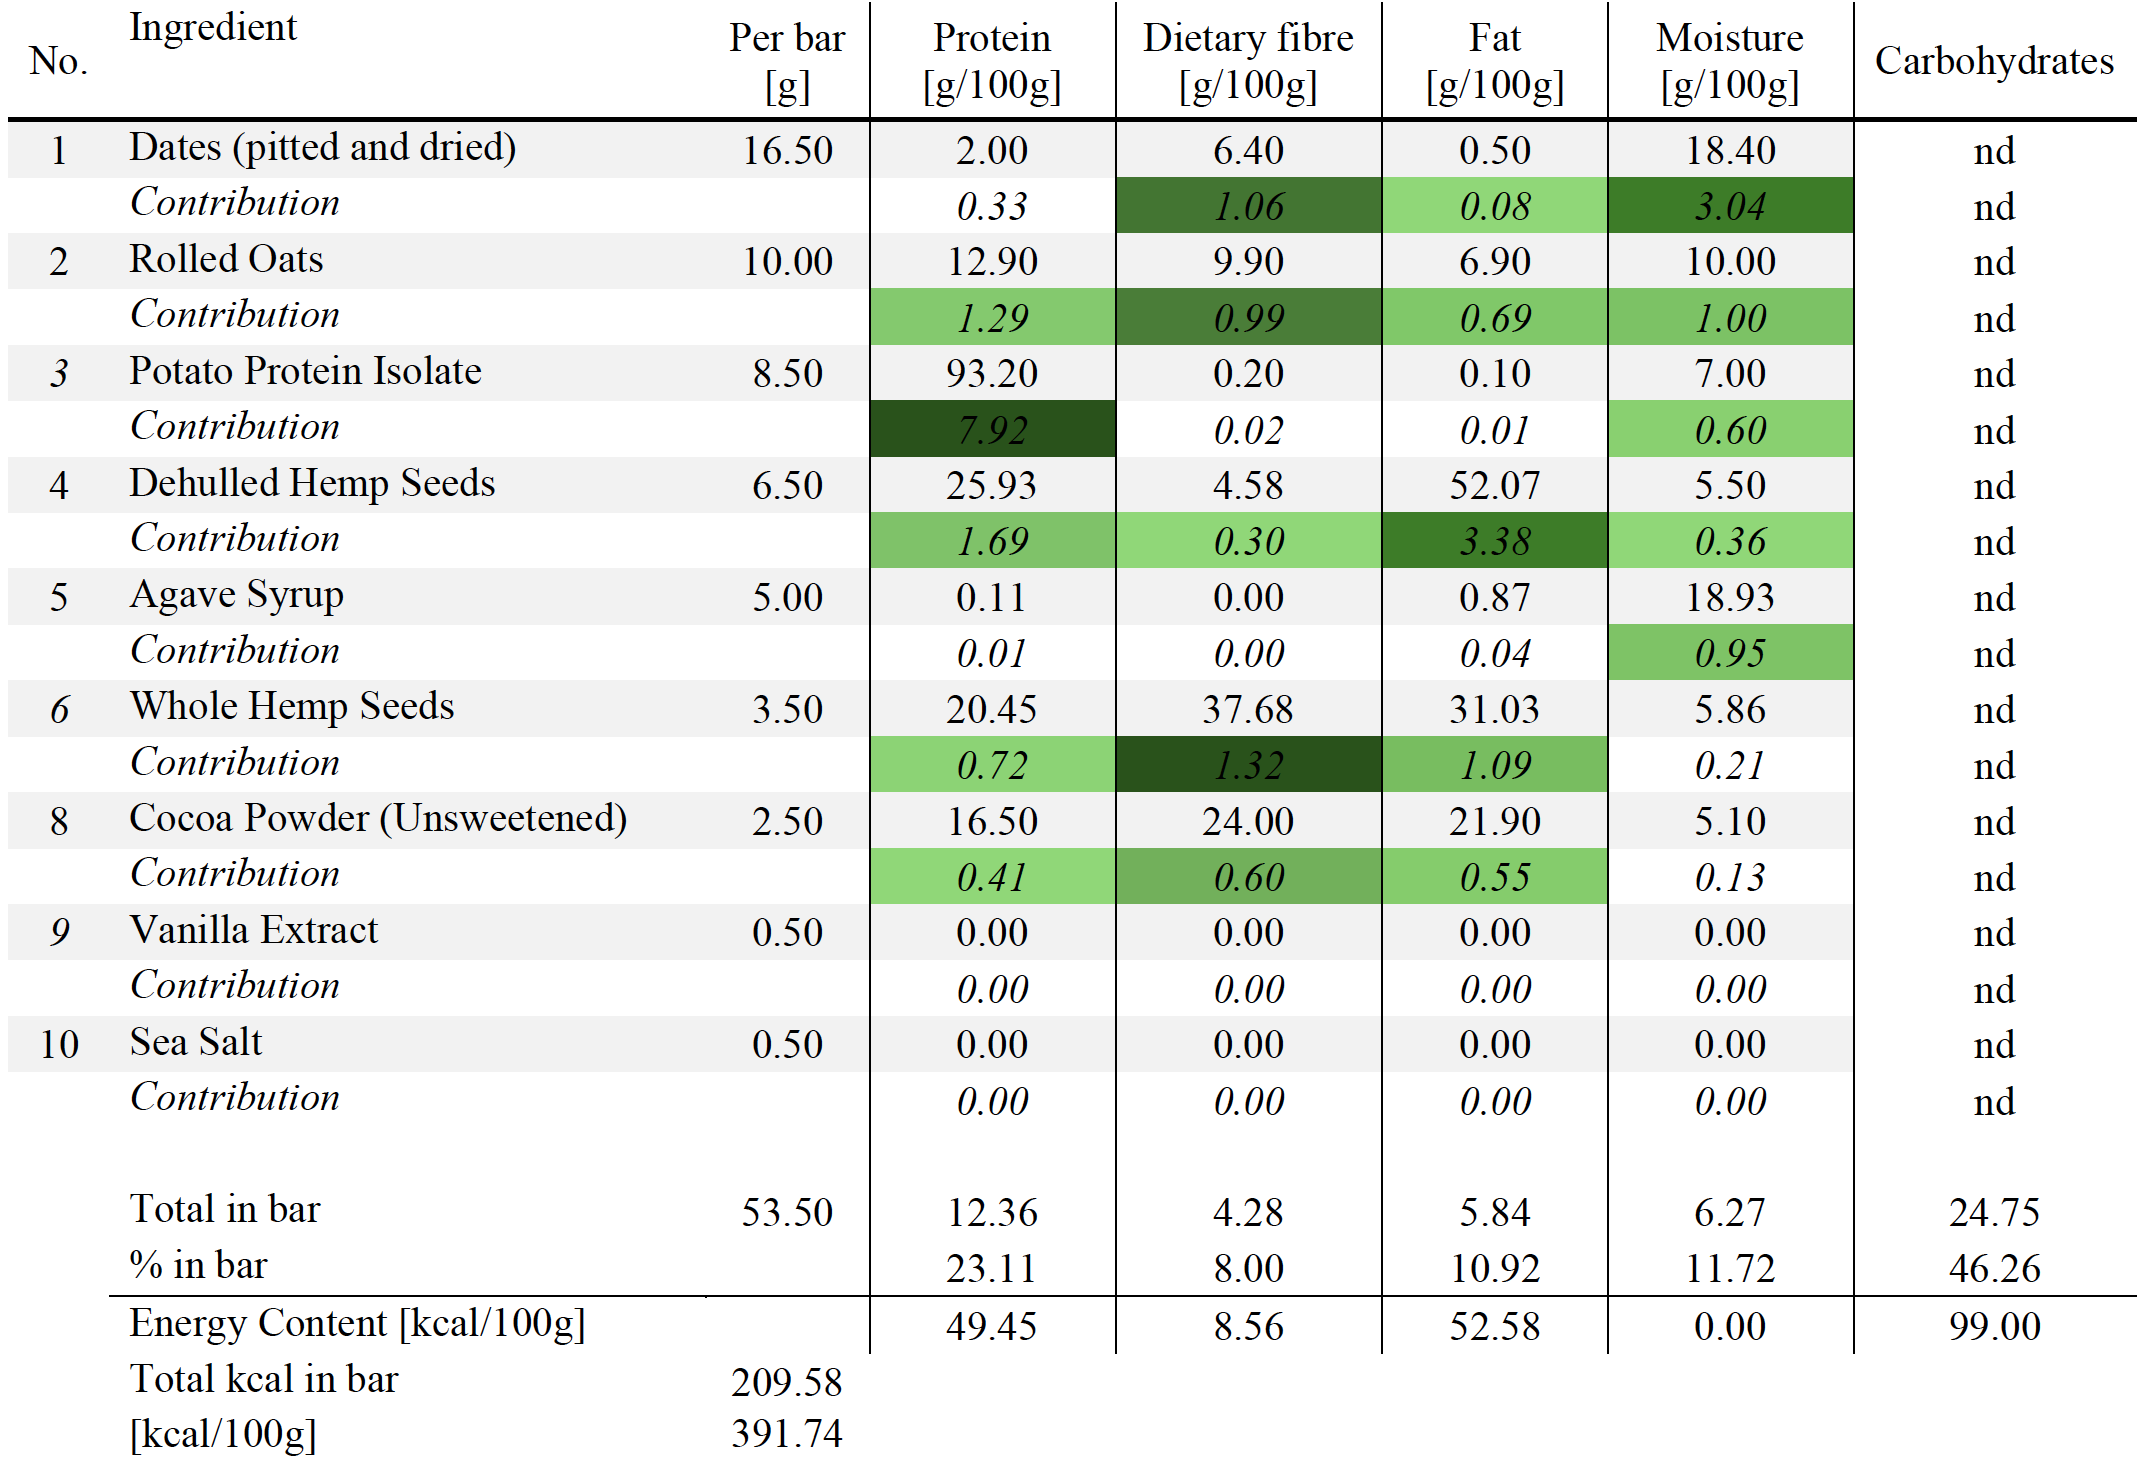
\includegraphics[width=\linewidth]{Figures/tab_overall_ingredients_01.png}
\end{table}

\subsection{Macronutrient Composition}
As shown in Table 6, the hemp seed protein bar delivers 209.6 kcal per 53.5 g bar, with a macronutrient profile characterised by 12.36 g protein, 4.28 g dietary fibre, 5.84 g fat, 6.27 g moisture, and 24.75 g carbohydrates. This balance between protein, fibre, and healthy fats underlines the bar’s potential as a nutrient-dense snack.

\vspace{1em}
The overall macronutrient profile was calculated using data from various sources to determine the contribution of each ingredient. For each raw material, published nutrient values were combined with the amount used per bar (g) to estimate the contribution of the respective ingredient. The calculations followed Equation 5.1. 


\begin{equation}
    \text{Contribution [g]} = 
    \frac{\text{Nutrient content [g/100g]} \times \text{Ingredient weight [g]}}{100}
    \label{eq:contribution}
\end{equation}

This approach was applied for protein, dietary fibre, fat and moisture. Carbohydrates were excluded from direct analysis, thus their content was derived by calculating the difference, as outlined in Equation 5.2. 

\begin{equation}
    \text{Carbohydrates [g]} = 
    \text{Total weight [g]} - (\text{Protein} + \text{Fat} + \text{Dietary fibre} + \text{Moisture})
    \label{eq:carbohydrates}
\end{equation}

The energy content of the bar was subsequently estimated while adhering to the conversions factors defined in regulation (EU) no. 1169/2011 (protein 4 kcal/g, carbohydrates 4 kcal/g, fibre 2 kcal/g) art\_17. The energy content for moisture was assumed to contribute with 0 kcal/g, thus neglected in the calculations. 

\vspace{1em}
Based on published nutrient values and the calculations described, the bar (53.5 g) provides 209.6 kcal, equivalent to 391.7 kcal/100 g. Its macronutrient composition - 23.1\% protein, 8.0\% dietary fibre, and 10.9\% fat - qualifies the product for the nutrition claims, “High protein” and “High fibre.” These claims comply with the conditions defined in the Annex of Regulation (EC) No 1924/2006, which governs nutrition and health claims across the European Union art\_16.    

\subsubsection{Protein Content and Quality}
Protein intake is essential for muscle protein synthesis, but the source and type of protein substantially influences its digestibility and utilisation. Since humans cannot synthesise essential amino acids, these must be obtained through diet. Consequently, the overall protein composition, and particularly the essential amino acids profile, is a key to determine protein quality art\_08.

\vspace{1em}
The hemp seed protein bar provides a total of 12.36 g protein per bar. As shown in Table 6, the main contributors for protein are potato protein isolate, rolled oats and dehulled hemp seeds. Dehulling is a processing step which has a significant effect on protein quality. It improves digestibility and reduces antinutritional factors, while also elevating the protein fraction of the hemp seed (hemp\_book). To further characterise the protein profile, Table 3 presents an in-depth analysis of the protein composition, with respect to each ingredient’s amino acid composition. The data was compiled from multiple sources, yet the methodologies used for amino acid determination has been similar across the studies (FridaFood, art\_08, art\_09, art\_10).

\vspace{1em}
The amino acid profile derived from the three main protein contributors includes all nine essential amino acids, confirming the bar as a complete protein source for the consumer. In each of the three main protein contributors, Leucine is the most abundant essential amino acid. Overall, Leucine makes up 5.32\% of the total amino acids contributed by the three ingredients. The combined amount of essential amino acids, derived from these contributors, amounts to 2568.83mg, of which Leucine alone constitutes 22.54\%.

\vspace{1em}
For both rolled oats, and dehulled hemps seeds, the lowest contribution stems from Tryptophan. General consensus, regarding the hemp seed amino acid profile identifies Lysine as the limiting essential amino acid. However, published values vary considerably depending on the analytical methods used, cultivation conditions and cultivar (hemp\_book). 

\vspace{1em}
Conversely, Tryptophan was not identified in published data for potato protein isolate, suggesting a scarce amounts present. For this ingredient, Methionine and Histidine was reported as the limiting essential amino acids, only contributing with 1300 mg/100g, which is substantially lower than the levels of the other essential amino acids. 

\vspace{1em}
The hemp seed protein bar exhibits an overall balanced essential amino acid profile, with only Tryptophan contributing under 1\% of the total amino acids, largely due to the absence of reported values in the potato protein isolate. The combination of the three main protein contributors therefore provides an amino acid profile, that can support several potential health benefits. In dehulled hemp seeds, Leucine, Phenylalanine, and Valine are three most abundant essential amino acids. Of these, only Valine is the only one not shared by the top three essential amino acid contributors in potato protein isolate. 

\vspace{1em}
Valine is one of the branched-chain amino acids (BCAAs), together with Isoleucine and leucine (art\_18). Elevated levels of Valine have been associated with various proposed benefits including improved weight gain, weight gain ratio, enhanced intestinal morphology, strengthened immune responses and increased bone density and strength (art\_19). As an essential amino acid, sufficient dietary intake is important, since valine is directly associated with protein synthesis and functions as a glucogenic amino acid within energy metabolism (art\_19). Although, valine itself has not been authorised any specific health claims under EU law, protein as a whole is recognised by EFSA to contribute to the maintenance and growth of muscle mass (art\_20).

\vspace{1em}
The combination of potato protein isolate, rolled oats, and dehulled hemp seeds enhances the amino acid profile, positioning the hemp protein bar as a sustainable and nutritionally valuable alternative to other conventional protein bars on the market. In addition, the presence of bioactive amino acids supports the bar’s functional value, making hemp a promising ingredient, as a source for high-quality plant protein.
    
\subsubsection{Dietary Fibre Content} 
Dietary fibres are carbohydrate polymers that cannot be absorbed in the human small intestine. These polymers, which contains three or more monomer units, have shown positive potential health benefits with significant prospect of improving carbohydrate metabolism and reducing cholesterol levels (art\_12\_01, art13\_02). In addition, certain dietary fibre factions act as prebiotics, and has shown physiological beneficial effects by supporting colonic fermentation and short-chain-fatty acids (art\_13\_02, art\_14). 

\vspace{1em}
The hemp seed protein bar provides a total of 4.28 g dietary fibre per bar. This corresponds to 8 g/100g which exceeds the conditions specified in the Annex of Regulation (EX) No. 1924/2006, for allowing a product to be labelled as “high fibre”.

% Is actually for the section above, but for layout reasons it has been inserted here.
\begin{table}[H]
    \caption{Amino acid composition of the three main protein-contributing ingredients in the hemp seed protein bar (rolled oats, potato protein isolate, and dehulled hemp seeds). The light orange rows indicate essential amino acids (EAAs). Within each amino acid column, the green shading represents relative contribution, ranging from light green (third highest contributor) to dark green (highest contributor). Red cells highlight the lowest contributing ingredient for that specific amino acid.}
\label{tab:df_amino_acids_01}
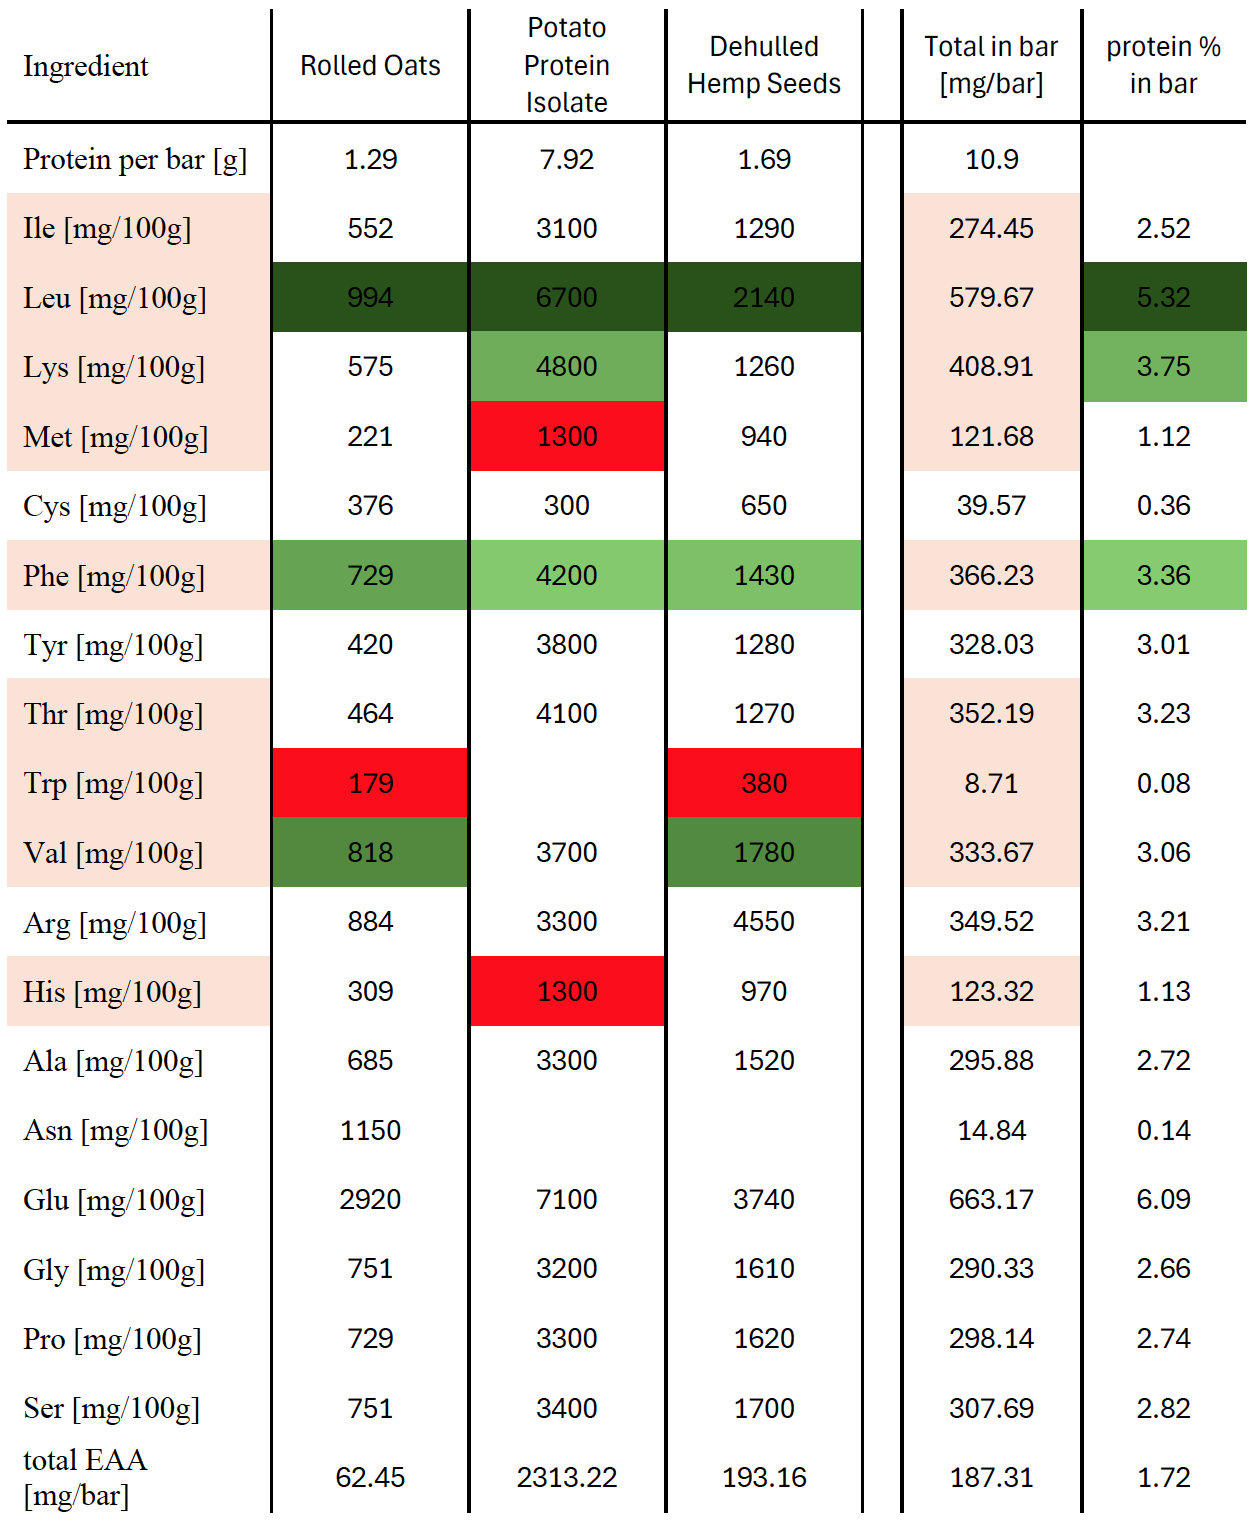
\includegraphics[width=\linewidth]{Figures/tab_amino_acid_01.png}
\end{table}

\vspace{1em}
As shown in Table 6, the main dietary fibre contributors of the hemp seed protein bar are whole hemp seeds, dates (pitted), and rolled oats, who each contributes with 1.32 g, 1.06 g, and 0.99 g, respectively. Processing also influences the dietary fibre profile of the ingredients. In oats, kilning has been used to inactivate lipase enzymes (art\_24), drying dates concentrates their fibre fractions while using whole hemp seeds (un-hulled) preserves their full dietary fibre content. Together, these three ingredients provide the majority of the dietary fibre in the product. When compared with the relative proportions in the product (Table 4), it can be noted, that whole hemp seeds, despite representing only 6.54\% of the bar’s weight, contributes the largest share of the total dietary fibre. Conversely, dates and rolled oats, which consist of 30.84\% and 18.69\% of the bar, respectively, provide less fibre relative to their much larger share of the formulation.

\vspace{1em}
Table 4 contains several blank entries, reflecting that not all ingredients contribute to each of the listed dietary fibre type, and that published data remain scarce, particularly for whole hemp seeds. Nevertheless, it is noteworthy that whole hemp seeds consistently display higher values g/100g for their respective fibre fractions. This highlights the role for whole hemp seeds as the most fibre-dense ingredient and the main contributor to the label “high fibre”. 

\vspace{1em}
The three main ingredients providing dietary fibres, contribute with a diverse palette of fibres. Whole hemp seeds mainly contribute with insoluble fibres such as cellulose, lignin, and hemicellulose. Rolled oats supply cellulose + $\beta-glucan$, lignin, and arabinoxylan, while dates provide these fraction as well as pectin. These fibres differ in solubility and fermentability, thus contributing to a complementary total dietary fibre profile of the hemp seed protein bar (art\_15).

\vspace{1em}
The data used for calculating the fibre fractions for both dates and rolled oats were obtained from published sources given as g/100g dry weight, and g/kg dry weight, respectively. In order to express these values on an as-is basis g/100g, the first step was to make a moisture content correction for the respective ingredients. These conversions were carried out according to Equation 3 and Equation 4, respectively. 


\begin{equation}
    x_{\text{as-is}}\!\left[\frac{\mathrm{g}}{100\,\mathrm{g}}\right]
    = x_{\mathrm{DW}}\!\left[\frac{\mathrm{g}}{100\,\mathrm{g}}\right]\cdot
    \bigl(1 - x_{\text{moisture}}\bigr)
    \label{eq:asis_simple}
\end{equation}

And

\begin{equation}
    x_{\text{as-is}}\!\left[\frac{\mathrm{g}}{100\,\mathrm{g}}\right]
    = \frac{\,x_{\mathrm{DW}}\!\left[\frac{\mathrm{g}}{100\,\mathrm{g}}\right]\,}{10}\,\cdot
    \bigl(1 - x_{\text{moisture}}\bigr)
    \label{eq:asis_div10}
\end{equation}
    
The values for the dietary fibre fractions for whole hemp seeds were given in \% of dry weight, so the calculation had to follow Equation 5.     

\begin{equation}
    x_{\text{as-is}}\!\left[\frac{\mathrm{g}}{100\,\mathrm{g}}\right]
    = \bigl( x_{\mathrm{DW}}\!\left[\tfrac{\mathrm{g}}{100\,\mathrm{g}}\right]
    \cdot (1 - x_{\text{moisture}}) \bigr)
    \cdot x_{\text{DFfraction}}
    \label{eq:asis_dffraction}
\end{equation}

These conversions (Equation 3-5) ensured that all reported values, despite differences in study and unit expression, were standardised to a consistent unit. This enabled a direct comparison between the fibre fractions contributed by the three ingredients. 



\subsubsection{Fatty Acid Profile}
The hemp seed protein bar has a total fat content of 5.84 g. The main contributors to this fat content
are dehulled hemp seeds, whole hemp seeds, and rolled oats, which contribute with 3.38 g, 1.09 g,
and 0.69 g, respectively, as shown in Table 6. Processing steps also affect the lipid quality.

\vspace{1em}
Processing steps also affect the lipid quality. Dehulling the hemp seeds increases the fat fraction by removing the hull mass. For a deeper insight into the specific fatty acid profile of the hemp protein bar, Table 5 was constructed to illustrate the distribution of fatty acid fractions from the top three ingredients. 

\begin{table}[H]
    \centering
    \caption{Contribution of the main dietary fibre sources (dates, rolled oats, and whole hemp seeds) to the hemp seed protein bar,
    expressed as total dietary fibre per bar and distribution of fibre fractions. Coloured cells indicate relative contribution, with light
    green representing lowest top three value and dark green representing the highest of the top three. The red coloured cells indicate the
    lowest value for each ingredient.}
    \label{tab:df_tab_01}
    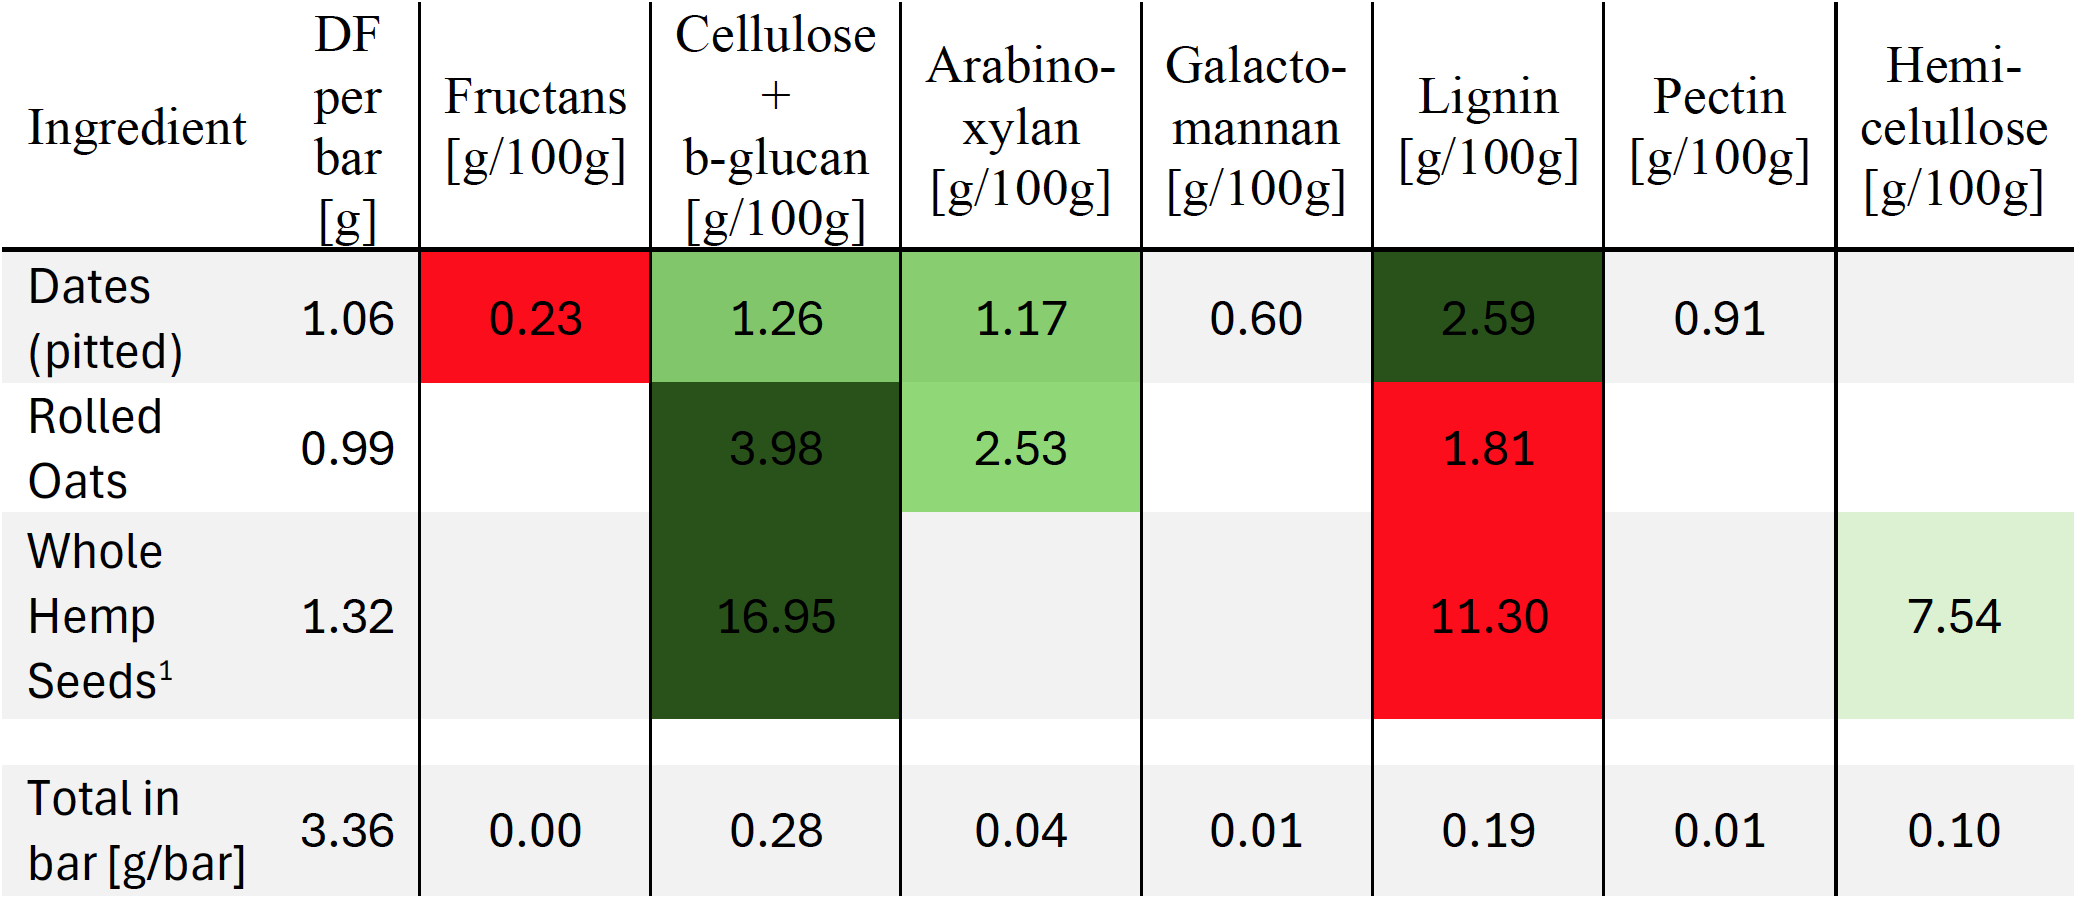
\includegraphics[width=\linewidth]{Figures/tab_df_01.png}
\end{table}

\vspace{1em}
It can be seen in Table 5, that the fatty acid profile is dominated by the polyunsaturated fatty acids (PUFAs). Notably, linoleic acid (LA, C18:2 n-6) and $\alpha$-linoleic acid (ALA, C18:3 n-3) constitutes 69.47\% of the total fatty acids quantified in the bar. These two essential fatty acids, LA (an omega-6) and ALA (an omega-3), cannot be synthetised by the human body and must therefore be obtained through diet. The abundance in the fatty acid profile highlights the nutritional value of the hemp protein bar. Previous studies have reported that LA and ALA from hemp seeds may the nervous system, supporting the health of blood vessels and to protect against cardiovascular diseases (art\_21). 

\vspace{1em}
Omega-6 tends to have pro-inflammatory pathways, whereas omega-3 supports anti-inflammatory responses. Therefore, maintaining an appropriate balance between these fatty acids is imperative (art\_21). Although EFSA does not prescribe a fixed omega-6 to omega-3 ratio, its Adequate Intake levels for LA (4\% of energy) and ALA (0.5\% of energy) imply a target ratio of approximately 3\:1. The hemp protein bar provides 1.022 g of omega-6 and 0.430 g of omega-3, yielding a ratio of 2.38\:1, close to, but slightly below the recommended guidelines (art\_22). 

\vspace{1em}
As stated, EFSA has set the Adequate Intake levels for LA and ALA to 4E\% and 0.5E\%, respectively. Based on a diet of 2000 kcal, this corresponds to approximately 8.9 g/day of LA and 1.1 g/day of ALA. 



\vspace{1em}
The hemp protein bar will provide roughly 11.5\% and 39\% of the daily requirements of LA and ALA, respectively. Although the substantial contribution to the daily fatty acid intake, these levels does not meet the conditions set by EU for nutrition and health claims. ALA falls below the $geq$ 0.3 g/100kcal threshold for the claim “source of omega-3 fatty acids” (art\_23), and LA remains below the $\geq$ 1.5 g/100kcal threshold requires for the claim “contributes to the maintenance of normal blood cholesterol levels” (art\_24).

\vspace{1em}
Saturated fatty acids (SFAs) in the hemp protein bar sum to 0.277g per bar, or 13.27\% of the total fatty acid profile. Palmitic acid (C16:0) is the predominant fraction, contributing with 0.199 g per bar. 
Monounsaturated fatty acids (MUFAs) account for 0.360 g of the hemp bar, representing 17.24\% of the 2.09 g total fatty acids. Table 5 illustrates that oleic acid (C18:1, n-9) is the dominant MUFA, consistently ranking among the three most abundant fatty acid fractions in dehulled hemp seeds, whole hemp seeds, and rolled oats. 


\begin{table}[H]
    \centering
    \caption{Contribution of the main dietary fibre sources (dates, rolled oats, and whole hemp seeds) to the hemp seed protein bar,
    expressed as total dietary fibre per bar and distribution of fibre fractions. Coloured cells indicate relative contribution, with light
    green representing lowest top three value and dark green representing the highest of the top three. The red coloured cells indicate the
    lowest value for each ingredient.}
    \label{tab:fatty_acid_tab_01}
    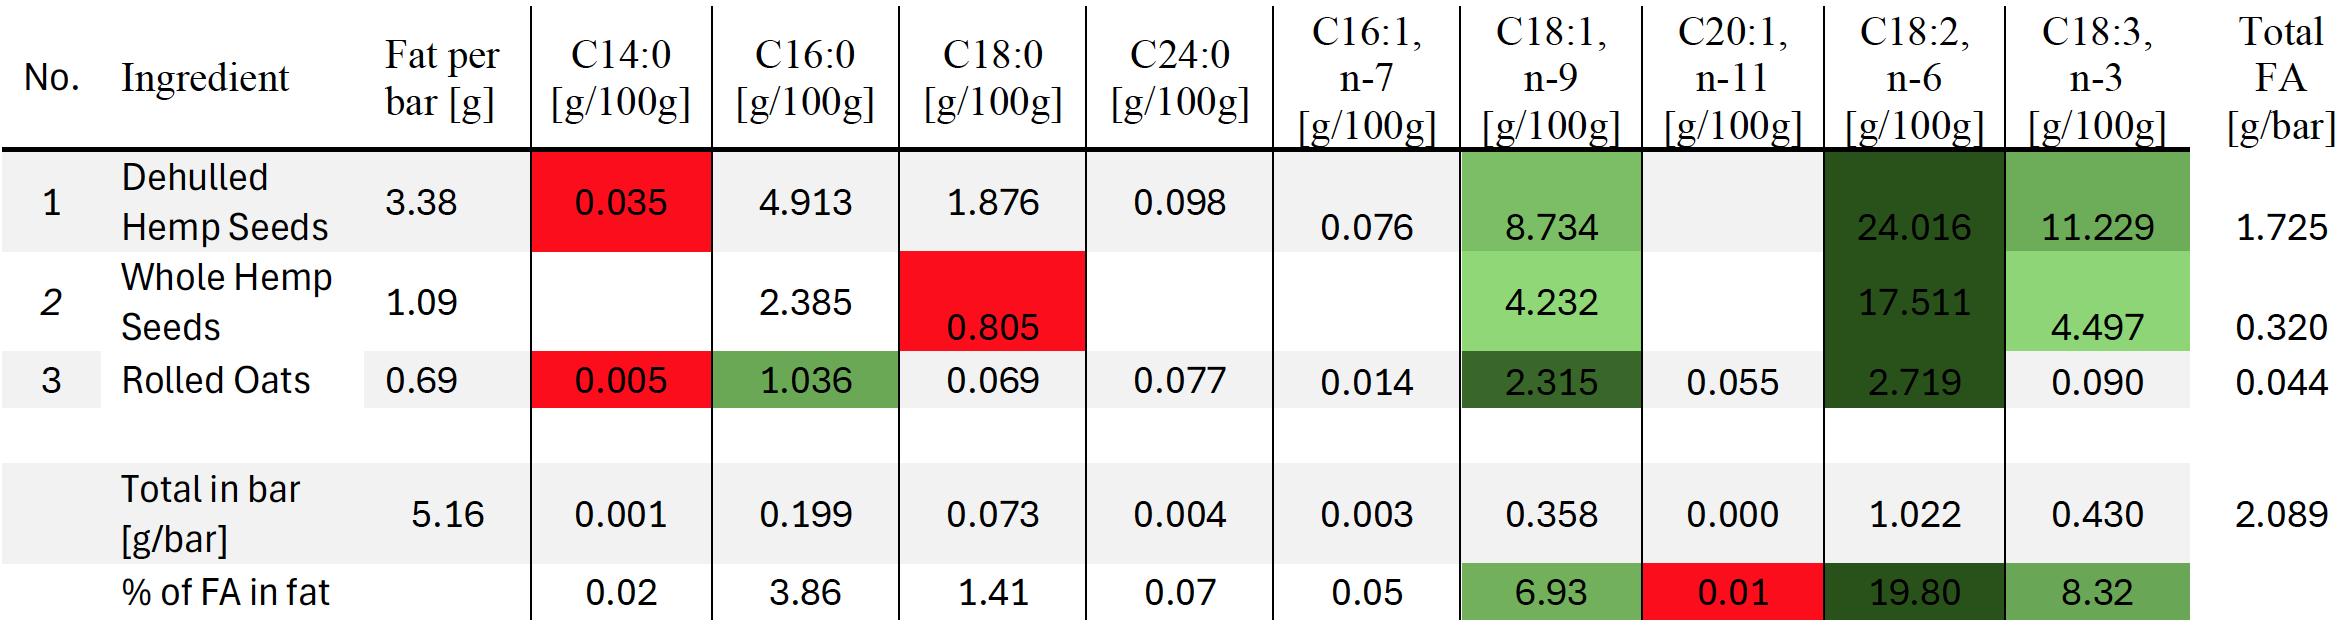
\includegraphics[angle=90,origin=c,width=0.23\textheight]{Figures/tab_fatty_01.png}
\end{table}




\newpage
\printbibliography[heading=bibsection]

% \begin{appendices}
%     \chapter{Appendix}
\section{Appendix 1 - GAI declaration}
\label{appendix1}
\includepdf[pages=-]{/Users/bruger/Desktop/Folders/KU/Master/year_2/blok_01/FBCPQ/individual_report/fbcpq_report/fbcpq_individual_project_files/Appendices/AI-declaration-ENG.pdf}

% \end{appendices}

\end{document}